\documentclass[1p,times,authoryear]{elsarticle}
\usepackage[usenames,dvipsnames]{xcolor}
\usepackage{wrapfig}
\usepackage{amssymb}
\usepackage{amsmath}
\usepackage{amssymb}
\usepackage{amsfonts}
\usepackage{amsthm}
\usepackage{float}
\usepackage{bm}
\usepackage{latexsym}
\usepackage{hyperref}
\usepackage[capitalize]{cleveref}
\usepackage{graphicx}
\usepackage{caption}
\usepackage{subcaption}
\usepackage{tikz}
\hypersetup{
    colorlinks,
    citecolor=blue,%    filecolor=black,%
    linkcolor=blue,     urlcolor=blue
}

% Use smaller margins
\usepackage{geometry}               	
\geometry{a4paper,margin=1.0in} 

\newcommand{\ir}{\frac{1}{r}}
\newcommand{\Integ}[1]{\int_{-\infty}^{\infty} \!\!\!\!\!\!
  \mathrm{d}#1}
\newcommand{\RInteg}[1]{\int_{0}^{\infty} \!\!\!\!\! #1\mathrm{d}#1}
\newcommand{\rInteg}{\int_{0}^{r_{max}} \!\!\!\!\! r\mathrm{d}r}
\newcommand{\TInteg}[1]{\int_{0}^{2\pi} \!\!\!\!\!\! \mathrm{d}#1}

\newcommand{\tB}[2]{\spectral{B}_{#1,m}^{#2}}
\newcommand{\tE}[2]{\spectral{E}_{#1,m}^{#2}}
\newcommand{\tj}[2]{\spectral{J}_{#1,m}^{#2}}

\newcommand{\trho}[1]{\spectral{\rho}_{m}^{#1}}

\renewcommand{\vec}[1]{\boldsymbol{#1}}

\newcommand{\comment}[1]{\textcolor{red}{#1}}

\newcommand{\spectral}[1]{\hat{\mathcal{#1}}}

% Reference automatique aux equations, sections, figures
\usepackage{cleveref}

\title{A spectral, quasi-cylindrical and dispersion-free Particle-In-Cell algorithm}
%\pagestyle{empty}
\author[label1]{R\'emi {Lehe}}
\ead{rlehe@lbl.gov}
\author[label2]{Manuel {Kirchen}}
\author[label3]{Igor A. {Andriyash}}
\author[label4]{Brendan B. {Godfrey}}
\author[label1]{Jean-Luc {Vay}}

\address[label1]{Lawrence Berkeley National Laboratory, Berkeley, CA 94720, USA}
\address[label2]{DESY, 22607 Hamburg, Germany}
\address[label3]{LOA, 91761 Palaiseau, France}
\address[label4]{University of Maryland, College Park, MD 20742, USA}

\begin{document}

\begin{abstract}
We propose a spectral Particle-In-Cell (PIC) algorithm which is based 
on the combination of a Hankel transform and a Fourier transform. 
For physical problems that have close-to-cylindrical symmetry, this
algorithm can be much faster than full 3D PIC algorithms. In addition,
unlike standard PIC algorithms, the proposed algorithm is free of numerical
dispersion. Morevover, this algorithm is benchmarked in several situations that
are of interest for the study of laser-plasma interactions. These
benchmarks show that the proposed algorithm 
avoids a number of numerical artifacts, that
would otherwise affect the physics in a standard PIC algorithm -- 
including the lowest-order numerical Cherenkov effect.
\end{abstract}

\maketitle

\section*{Introduction}

Particle-In-Cell (PIC) algorithms \citep{Birdsall2004,Hockney1988} 
are extensively used in several areas of physics, including the study
of astrophysical plasmas, fusion plasmas, laser-plasma
interactions and accelerator physics. Yet,
despite their wide use, PIC algorithms remain very computationally
demanding and are still subject to a range of numerical artifacts. 
These shortcomings can be particularly significant when simulating 
accelerated particle beams, or 
laser-plasma interactions (such as laser-wakefield acceleration). 
This is mainly for two reasons:
\begin{itemize}
\item In these particular cases, the system often has close-to-cylindrical
  symmetry (e.g. particle beams and laser pulses are often
  cylindrically symmetric). This prevents the use of 2D Cartesian 
PIC algorithms (which are only well-suited for slab-like symmetry),
and is instead often dealt with by using
  3D Cartesian PIC algorithms. However, 3D PIC algorithms are extremely
  computationally intensive.
\item The physical objects of interest (e.g. the laser, or the
  accelerated particle beam) often propagate close to the speed of
  light. This makes them very sensitive to \emph{numerical
    dispersion}, i.e. the fact that the electromagnetic waves do not
  propagate exactly at the physical speed of light in a standard PIC
  code, but propagate instead at a spuriously-altered,
  resolution-dependent speed. In the above-mentioned cases, 
numerical dispersion can lead to substantial numerical artifacts
which can mask or disrupt the physics at stake in the simulation. This
includes for instance numerical Cherenkov effect in general
\citep{GodfreyJCP1974}, but also more specific artifacts, such as
e.g. the erroneous prediction of the dephasing length in
laser-wakefield acceleration \citep{CowanPRSTAB2013}.

\end{itemize}
Yet several improvements can be made to the PIC algorithm, in order
to mitigate these difficulties and increase the speed and
accuracy of the simulations in these situations. 
\begin{itemize}
\item One of these improvements is the recent
  development of cylindrically-symmetric
PIC algorithms with azimuthal Fourier decomposition \citep{Lifschitz,Davidson} 
(sometimes refered to as \emph{quasi-3D} algorithms, or
\emph{quasi-cylindrical} algorithms as we do here). By taking
into account the symmetry of the system, these algorithms can typically reduce
the cost of the simulation to a few times that of a 2D Cartesian simulation,
instead of that of a full 3D Cartesian simulation. Moreover, unlike 2D
Cartesian algorithms, these algorithms are well adapted to close-to-cylindrical
physical systems and can accurately capture physical effects that are intrisically
3D (such as e.g. the non-linear self-focusing of an intense laser in a
plasma \citep{EsareyRMP2009}).

\item A second, separate improvement was introduced by the development
  of \emph{spectral} Cartesian PIC algorithms
  \citep{BunemanJCP1980,DawsonRMP1983} i.e. algorithms that solve the
  Maxwell equations in Fourier space. These algorithms contrast with
  \emph{finite-difference} algorithms, which solve the Maxwell equations
  by approximating the derivatives as finite differences on a discrete spatial grid.
Importantly, while finite-difference algorithm often strongly suffer from
numerical dispersion, there is a class of spectral algorithms -- often refered to
as \emph{Pseudo-Spectral Analytical Time Domain} (PSATD) algorithms 
\citep{Haber} -- which exhibits no numerical dispersion whatsoever. As a
consequence, these algorithms are free from the numerical artifacts
associated with the spurious speed of the electromagnetic waves in PIC
codes. Moreover, it was shown recently
\citep{XuJCP2013,YuJCP2014,YuCPC2015,
GodfreyIEEE2014,GodfreyJCP2014} 
that spectral PIC algorithms have better stability properties when 
performing PIC simulations in
a Lorentz-boosted frame \citep{VayPRL2007,MartinsNatPhys2010}. 
These stability properties are very
promising since boosted-frame simulations can be faster than 
their laboratory-frame counterparts by several orders of magnitude \citep{VayPRL2007}.
\end{itemize}

Even though these two improvements are both very valuable, they cannot be
combined with one another in their present
formulation. This is because the \emph{quasi-cylindrical} algorithm uses a
cylindrical system of coordinates, whereas the spectral PIC algorithms
(and in particular the \emph{PSTAD} algorithms)
were developped in a Cartesian system of coordinates. This
incompatibility is however not definitive, and the aim of this article
is to overcome these differences by developping a \emph{spectral
  quasi-cylindrical} formalism. In this document, we derive this formalism,
and we show that it can be used to build a PIC algorithm that combines 
the speed of \emph{quasi-cylindrical} algorithms with
the accuracy and lack of numerical dispersion of the \emph{PSATD} algorithms.

Although the algorithm described here is, to our knowledge, unique in
its capabilities, there are several other PIC algorithms that use 
a similar -- yet not equivalent -- approach. One such example is the
hybrid, quasi-cylindrical version of \textsc{OSIRIS} \citep{Yuarxiv2015}. This algorithm
involves a Fourier transform in the longitudinal direction, but
retains a finite-difference formulation in the transverse (radial)
direction. As a consequence, this algorithm is not fully spectral, nor
fully dispersion-free. Another such example is the PIC code \textsc{PlaRes} 
\citep{AndriyashJCP2015}, which also uses a spectral quasi-cylindrical
formalism but relies on the scalar and vector potentials
$\phi$ and $\vec{A}$ instead of the standard PIC formulation in terms
of $\vec{E}$ and $\vec{B}$. As a result, \textsc{PlaRes} largely differs from the
algorithm described here, both in the equations that it simulates and
in their numerical implementation.

In the present article, we start by deriving the equations of our
spectral quasi-cylindrical formalism (\cref{sec:theory}). We then explain
how these equations were discretized and implemented in a fully
working PIC code (\cref{sec:implementation}). We then report on the
results of a number of benchmarks that were performed with this PIC
code (\cref{sec:benchmarks}), and describe two typical physical situations in
which our spectral algorithm performs better than standard 
finite-difference algorithms (\cref{sec:advantages}).

\section{Representation of the fields and continuous equations}
\label{sec:theory}

\subsection{A reminder on spectral Cartesian codes}

It is well-known that the Maxwell equations in Cartesian coordinates 
\begin{align}
\frac{1}{c^2}\partial_t E_x = \partial_y B_z - \partial_z B_y - \mu_0  j_x \qquad&   
\partial_t B_x = -\partial_y E_z + \partial_z E_y \label{eq:CartMaxwellx} \\
\frac{1}{c^2}\partial_t E_y = \partial_z B_x - \partial_x B_z - \mu_0  j_y \qquad &   
\partial_t B_y = -\partial_z E_x + \partial_x E_z \label{eq:CartMaxwelly}  \\
\frac{1}{c^2}\partial_t E_z = \partial_x B_y - \partial_y B_x - \mu_0  j_z \qquad &   
\partial_t B_z = -\partial_x E_y + \partial_y E_x \label{eq:CartMaxwellz} 
\end{align}
can be solved by representing the fields as a sum of Fourier modes.
\begin{equation}
\label{eq:CartBwTrans}
F_u(\vec{r}) = \frac{1}{(2\pi)^{3}}\Integ{k_x} \,\Integ{k_y}\,
\Integ{k_z} \; \mathcal{F}_u(\vec{k}) \, e^{i(k_x x + k_y y + k_z z)} 
\end{equation}
with 
\begin{equation}
\label{eq:CartFwTrans}
\mathcal{F}_u(\vec{k})  = \Integ{x} \,\Integ{y}\, \Integ{z} \;
F_u(\vec{r}) \, e^{-i(k_x x + k_y y + k_z z)} 
\end{equation}
where $F$ is any of the fields $E$, $B$ or $j$, and where $u$ is
either $x$, $y$ or $z$. $\mathcal{F}$ represents the Fourier
components of $F$, which will be denoted
$\mathcal{E}$, $\mathcal{B}$ or $\mathcal{J}$ depending on whether
$F$ represents $E$, $B$ or $j$. With this representation, the
different Fourier modes decouple and the equations 
\cref{eq:CartMaxwellx,eq:CartMaxwelly,eq:CartMaxwellz} become 
\begin{align}
\frac{1}{c^2}\partial_t \mathcal{E}_x = ik_y \mathcal{B}_z - ik_z \mathcal{B}_y - \mu_0 \mathcal{J}_x \qquad &   
\partial_t \mathcal{B}_x = -ik_y \mathcal{E}_z + ik_z \mathcal{E}_y \label{eq:CartSpectMaxwellx}\\
\frac{1}{c^2}\partial_t \mathcal{E}_y = ik_z \mathcal{B}_x - ik_x \mathcal{B}_z - \mu_0  \mathcal{J}_y \qquad &   
\partial_t \mathcal{B}_y = -ik_z \mathcal{E}_x + ik_x \mathcal{E}_z \label{eq:CartSpectMaxwelly}\\
\frac{1}{c^2}\partial_t \mathcal{E}_z = ik_x \mathcal{B}_y - ik_y \mathcal{B}_x - \mu_0 \mathcal{J}_z  \qquad &   
\partial_t \mathcal{B}_z = -ik_x \mathcal{E}_y + ik_y \mathcal{E}_x \label{eq:CartSpectMaxwellz}
\end{align}
The Fourier coefficients can then be integrated in time, and
transformed back into real space using \cref{eq:CartBwTrans}. This is
the core principle of spectral Cartesian algorithms, including the PSATD algorithms.

\subsection{Spectral quasi-cylindrical representation}

The Fourier representation \cref{eq:CartBwTrans} is no longer the
appropriate representation when the Maxwell equations are written in cylindrical coordinates.
\begin{align}
\frac{1}{c^2}\partial_t E_r = \ir \partial_\theta B_z - \partial_z B_\theta - \mu_0  j_r \qquad&   
\partial_t B_r = -\ir \partial_\theta E_z + \partial_z E_\theta \label{eq:CircMaxwellr} \\
\frac{1}{c^2}\partial_t E_\theta = \partial_z B_r - \partial_r B_z - \mu_0  j_\theta \qquad &   
\partial_t B_\theta = -\partial_z E_r + \partial_r E_z \label{eq:CircMaxwellt}  \\
\frac{1}{c^2}\partial_t E_z = \ir\partial_r r B_\theta - \ir\partial_\theta B_r - \mu_0  j_z \qquad & 
\partial_t B_z = -\ir\partial_r r E_\theta + \ir\partial_\theta E_r \label{eq:CircMaxwellzz} 
\end{align}
When replacing
\cref{eq:CartBwTrans} into the \cref{eq:CircMaxwellr,eq:CircMaxwellt,eq:CircMaxwellzz}, the Fourier modes do not decouple. Instead one has to use the Fourier-Bessel representation.
\begin{align}
& F_z(\vec{r}) = \frac{1}{(2\pi)^2}\!\!\!\sum_{m=-\infty}^{\infty} \Integ{k_z}
\RInteg{k_\perp }\; \spectral{F}_{z,m}(k_z,k_\perp ) \; J_m(k_\perp r)\, e^{-im\theta + ik_z z} 
\label{eq:CircBwTransz} \\
& F_r(\vec{r}) = \frac{1}{(2\pi)^2}\!\!\!\sum_{m=-\infty}^{\infty} \Integ{k_z}\,\RInteg{k_\perp }\;
\left( \spectral{F}_{+,m}(k_z,k_\perp )\; J_{m+1}(k_\perp r) +\spectral{F}_{-,m}(k_z,k_\perp )\; J_{m-1}(k_\perp r)
\right)  e^{-im\theta +ik_z z}
\label{eq:CircBwTransr} \\
& F_\theta(\vec{r}) = \frac{1}{(2\pi)^2}\!\!\!\sum_{m=-\infty}^{\infty} \Integ{k_z}\,\RInteg{k_\perp }\;
i\left( \spectral{F}_{+,m}(k_z,k_\perp )\; J_{m+1}(k_\perp r) - \spectral{F}_{-,m}(k_z,k_\perp )\; J_{m-1}(k_\perp r)
\right)  e^{-im\theta +ik_z z} 
\label{eq:CircBwTranst}
\end{align}
where $F$ is either $E$, $B$ or $j$, where $J_m$ denotes the Bessel
function of order $m$, and where $\spectral{F}_{z,m}$, $\spectral{F}_{+,m}$ and
 $\spectral{F}_{-,m}$ represent the spectral components of $F$. These spectral components are given by:
\begin{align}
\spectral{F}_{z,m}(k_z,k_\perp ) &= \Integ{z} \RInteg{r}
\TInteg{\theta} \;F_z(\vec{r})\; J_m(k_\perp r) e^{im\theta
 - i k_z z} \label{eq:CircFwTransz} \\
\spectral{F}_{+,m}(k_z,k_\perp ) &= \Integ{z} \RInteg{r}
\TInteg{\theta} \;\frac{F_r (\vec{r})-iF_\theta (\vec{r})}{2}\; J_{m+1}(k_\perp r) e^{im\theta
 - i k_z z} \label{eq:CircFwTransp} \\
\spectral{F}_{-,m}(k_z,k_\perp ) &= \Integ{z} \RInteg{r}
\TInteg{\theta} \;\frac{F_r (\vec{r})+iF_\theta(\vec{r})}{2}\; J_{m-1}(k_\perp r) e^{im\theta
 - i k_z z} \label{eq:CircFwTransm} 
\end{align}
\noindent Notice here that the Cartesian
component $F_z$ and cylindrical components
$F_r$, $F_\theta$ do not transform in the same manner, which is due
to their different behavior close to the axis. (See
\ref{sec:CircTrans} for a derivation of the above equations.) 
Note also that scalar fields (like $\rho$) transform in the
same way as the Cartesian component $F_z$. 

When replacing \cref{eq:CircBwTransr,eq:CircBwTranst,eq:CircBwTransz} into the Maxwell equations in cylindrical
coordinates \cref{eq:CircMaxwellr,eq:CircMaxwellt,eq:CircMaxwellzz},
the different modes decouple, and the equations for the spectral
coefficients become:
\begin{align}
\frac{1}{c^2}\partial_t \spectral{E}_{+,m} = - \frac{ik_\perp }{2}\spectral{B}_{z,m} + k_z\spectral{B}_{+,m} - \mu_0\spectral{J}_{+,m} \qquad &   
\partial_t \spectral{B}_{+,m} = \frac{ik_\perp }{2} \spectral{E}_{z,m} - k_z
\spectral{E}_{+,m} 
\label{eq:CircMaxwellp} \\
\frac{1}{c^2}\partial_t \spectral{E}_{-,m} = -\frac{ik_\perp }{2} \spectral{B}_{z,m} - k_z \spectral{B}_{-,m} - \mu_0  \spectral{J}_{-,m} \qquad &   
\partial_t \spectral{B}_{-,m} = \frac{ik_\perp }{2} \spectral{E}_{z,m} + k_z
\spectral{E}_{-,m} \label{eq:CircMaxwellm} \\
\frac{1}{c^2}\partial_t \spectral{E}_{z,m} = ik_\perp  \spectral{B}_{+,m} + ik_\perp \spectral{B}_{-,m}  - \mu_0 \spectral{J}_{z,m}  \qquad & 
\partial_t \spectral{B}_{z,m} = -ik_\perp  \spectral{E}_{+,m} - ik_\perp \spectral{E}_{-,m}  \label{eq:CircMaxwellz} 
\end{align}
(See \ref{sec:SpectMaxwell} for a derivation of these equations.)
Notice that these equations have a similar structure as 
\cref{eq:CartSpectMaxwellx,eq:CartSpectMaxwelly,eq:CartSpectMaxwellz}, as 
they also involve the product of the fields with the components of
$\vec{k}$, in their right-hand side. They do differ however in their
details, as evidenced by the signs, the factors 1/2 and the
presence or absence of the complex number $i$ in some terms.

Similarly, in this formalism, the conservation equations
$\vec{\nabla}\cdot\vec{E}=\rho/\epsilon_0$ and
$\vec{\nabla}\cdot\vec{B} = 0$
become
\begin{equation}
\label{eq:SpectCons}
k_\perp (\spectral{E}_{+,m} -\spectral{E}_{-,m}) + ik_z \spectral{E}_{z,m} =
\frac{\spectral{\rho}_m}{\epsilon_0} \qquad
 k_\perp (\spectral{B}_{+,m} -\spectral{B}_{-,m}) + ik_z \spectral{B}_{z,m} =
0 \end{equation}
As expected, the above conservation equations are
preserved by the Maxwell equations
\cref{eq:CircMaxwellp,eq:CircMaxwellm,eq:CircMaxwellz}, provided
that the current satisfies $\partial_t
\rho + \vec{\nabla} \cdot \vec{j} = 0$, i.e. in spectral space:
\begin{equation}
\label{eq:SpectCharge}
\partial_t \spectral{\rho}_m + k_\perp (\spectral{J}_{+,m} -\spectral{J}_{-,m}) + ik_z
\spectral{J}_{z,m} = 0
\end{equation}  

As in a spectral Cartesian PIC codes, the equations
\cref{eq:CircMaxwellp,eq:CircMaxwellm,eq:CircMaxwellz}  
can be integrated in time, and the fields can then be transformed back into
real space, using \cref{eq:CircBwTransz,eq:CircBwTransr,eq:CircBwTranst}. Therefore,
the methods used to integrate the fields in time in a spectral Cartesian
code (e.g. PSATD) should be transposable to this spectral quasi-cylindrical formalism.

However, the advantage of this formalism over its Cartesian
counterpart is that the sum over $m$ in
\cref{eq:CircBwTransz,eq:CircBwTransr,eq:CircBwTranst} can generally
be truncated to only a few terms, for physical situations that have
close-to-cylindrical symmetry \citep{Lifschitz}. This is because the
different values of $m$ correspond to different azimuthal modes of the
form $e^{-im\theta}$, and because these modes are typically zero for
large values of $|m|$, in situations with close-to-cylindrical symmetry.
As a result, the representation of the fields is
reduced to a few 2D arrays $\spectral{F}_m(k_z,k_\perp )$ instead of the
Cartesian 3D arrays $\mathcal{F}(k_x,k_y,k_z)$. This reduction makes
the manipulation of the fields much more computationally efficient.

\section{Numerical implementation}
\label{sec:implementation}

\subsection{Overview of the algorithm}

The PIC algorithm described here uses the above-mentioned representation
of the fields. Although the fields are represented by a few
2D arrays, the particles are still distributed in 3D and their motion
is integrated in 3D Cartesian coordinates. However, due to the
lower number of cells in a 2D array, one can drastically reduce the
total number of particles and still have significative statistics for
each cell.

Similarly to a spectral Cartesian code, we do not perform the
current deposition and field gathering directly from the
macroparticles to the spectral space. (This is inefficient since the
deposition and gathering are local operations in real space -- i.e. affect
only the few cells next to the macroparticle -- but global operations
in spectral space -- i.e. they affect all the spectral modes
simultaneously.) Instead we use an intermediate grid where these
operations can be performed locally, and where the fields $\hat{F}_{u,m}$
are defined by
\begin{equation} 
\label{eq:IntermBwTrans}
F_u(\vec{r}) = \sum_{m=-\infty}^{\infty} \hat{F}_{u,m}(r,z)
e^{-im\theta} 
\end{equation}
\begin{equation}
\label{eq:IntermFwTrans}
\hat{F}_{u,m}(r,z) = \frac{1}{2\pi} \TInteg{\theta} \;
F_u(\vec{r})e^{im\theta}
\end{equation}
where ${F}$ is either ${E}$, ${B}$ or
${j}$ and $u$ is either $z$, $r$ or $\theta$. Notice that this representation is the
same as that of \citep{Lifschitz, Davidson}. In this
representation, the spectral decomposition in the azimuthal
direction is preserved, since the factors $e^{im\theta}$ can be efficiently computed from the
particle Cartesian positions $x,y,z$ by using the relation $e^{im\theta} = (x+iy)^m/r^m$
\citep{Lifschitz}.

After the particles deposit their charge and current onto this
intermediate grid, the fields of the grid are transformed into spectral
space where the Maxwell equations can be easily integrated. From
\cref{eq:IntermFwTrans,eq:IntermBwTrans} and
\cref{eq:CircFwTransz,eq:CircFwTransp,eq:CircFwTransm,eq:CircBwTransz,eq:CircBwTransr,eq:CircBwTranst}, 
the transformation between the intermediate grid $\hat{F}_{m}(r,z)$
and the spectral grid $\spectral{F}_m(k_\perp, k_z)$ is:
\begin{align}
\spectral{F}_{z,m}(k_\perp,k_z) & = \mathrm{HT}_{m} [ \; \mathrm{FT}
                               [ \; \hat{F}_{z,m}(r,z) \; ] \;] \\
\spectral{F}_{+,m}(k_\perp,k_z) &= \mathrm{HT}_{m+1}\left[ \; \mathrm{FT} \left[ \frac{
  \hat{F}_{r,m} -i  \hat{F}_{\theta,m} }{2}  \right] \;\right] \\
\spectral{F}_{-,m}(k_\perp,k_z) &= \mathrm{HT}_{m-1} \left[ \;\mathrm{FT} \left[ \frac{
  \hat{F}_{r,m} +i  \hat{F}_{\theta,m} }{2}  \right] \;\right] 
\end{align}
and
\begin{align}
\hat{F}_{z,m}(r,z) &= \mathrm{IFT} [\; \mathrm{IHT}_{m} [
                         \spectral{F}_{z,m}(k_\perp,k_z) ] \; ] \\
\hat{F}_{r,m}(r,z) & = \mathrm{IFT} \left[ \; \mathrm{IHT}_{m+1}
                         [ \spectral{F}_{+,m}(k_\perp,k_z) ] + \mathrm{IHT}_{m-1} [
                         \spectral{F}_{-,m}(k_\perp,k_z) ] \; \right] \label{eq:FTHTr}\\
\hat{F}_{\theta,m}(r,z) & = i\;\mathrm{IFT} \left[ \; \mathrm{IHT}_{m+1}
                         [ \spectral{F}_{+,m}(k_\perp,k_z) ] -
                          \mathrm{IHT}_{m-1} [
                          \spectral{F}_{-,m}(k_\perp,k_z) ] \; \right]
\label{eq:FTHTt}
\end{align}
where $\mathrm{FT}$ represents a Fourier Transform along the $z$
axis and $\mathrm{HT}_{n}$ represents a Hankel Transform of order
$n$ along the transverse $r$ axis, and where $\mathrm{IFT}$ and
$\mathrm{IHT}_{n}$ represent the corresponding inverse
transformations:
\[ \mathrm{FT} [f]\, (k_z) \equiv \Integ{z} \, e^{-ik_zz} \; f(z) \qquad 
\mathrm{IFT} [g] \,(z)\equiv \frac{1}{2\pi}\Integ{k_z} \, e^{ik_zz} \;  g(k_z)\]
\[ \mathrm{HT}_{n} [f]\,(k_\perp) \equiv 2\pi \RInteg{r} \,
J_{n}(k_\perp r) \; f(r) \qquad 
\mathrm{IHT}_{n} [g]\,(r) \equiv \frac{1}{2\pi}\RInteg{k_\perp} \,  J_{n}(k_\perp r)  \;  g(k_\perp) \]

The above equations show that the transformation from the intermediate
grid ($\hat{F}_{u,m}$) to the spectral grid ($\spectral{F}_{u,m}$) is
the combination of a Fourier transform (in $z$) and a Hankel transform
(in $r$). The Fourier transform in $z$ can be implemented through a Fast Fourier
Transform (FFT) algorithm, which imposes to use an evenly-spaced grid
in $z$ and in $k_z$. On the other hand, there is more freedom of
choice for the Discrete Hankel Transform (DHT), and the implementation that
we chose is described in the next section
(\cref{sec:discretization}) and in the \ref{sec:HTMatrix}.

\Cref{fig:GlobalScheme} gives an overview of the successive steps
involved in one PIC cycle, including the
respective role of the intermediate and spectral grid. Note that, in the PSATD
scheme that we chose (and which is described in more details in
\cref{sec:FieldIntegration}), all the fields are defined at integer
timesteps, except for the currents, which are defined at half
timesteps. The following subsections describe the successive steps of
the PIC cycle in more details.

\begin{figure}

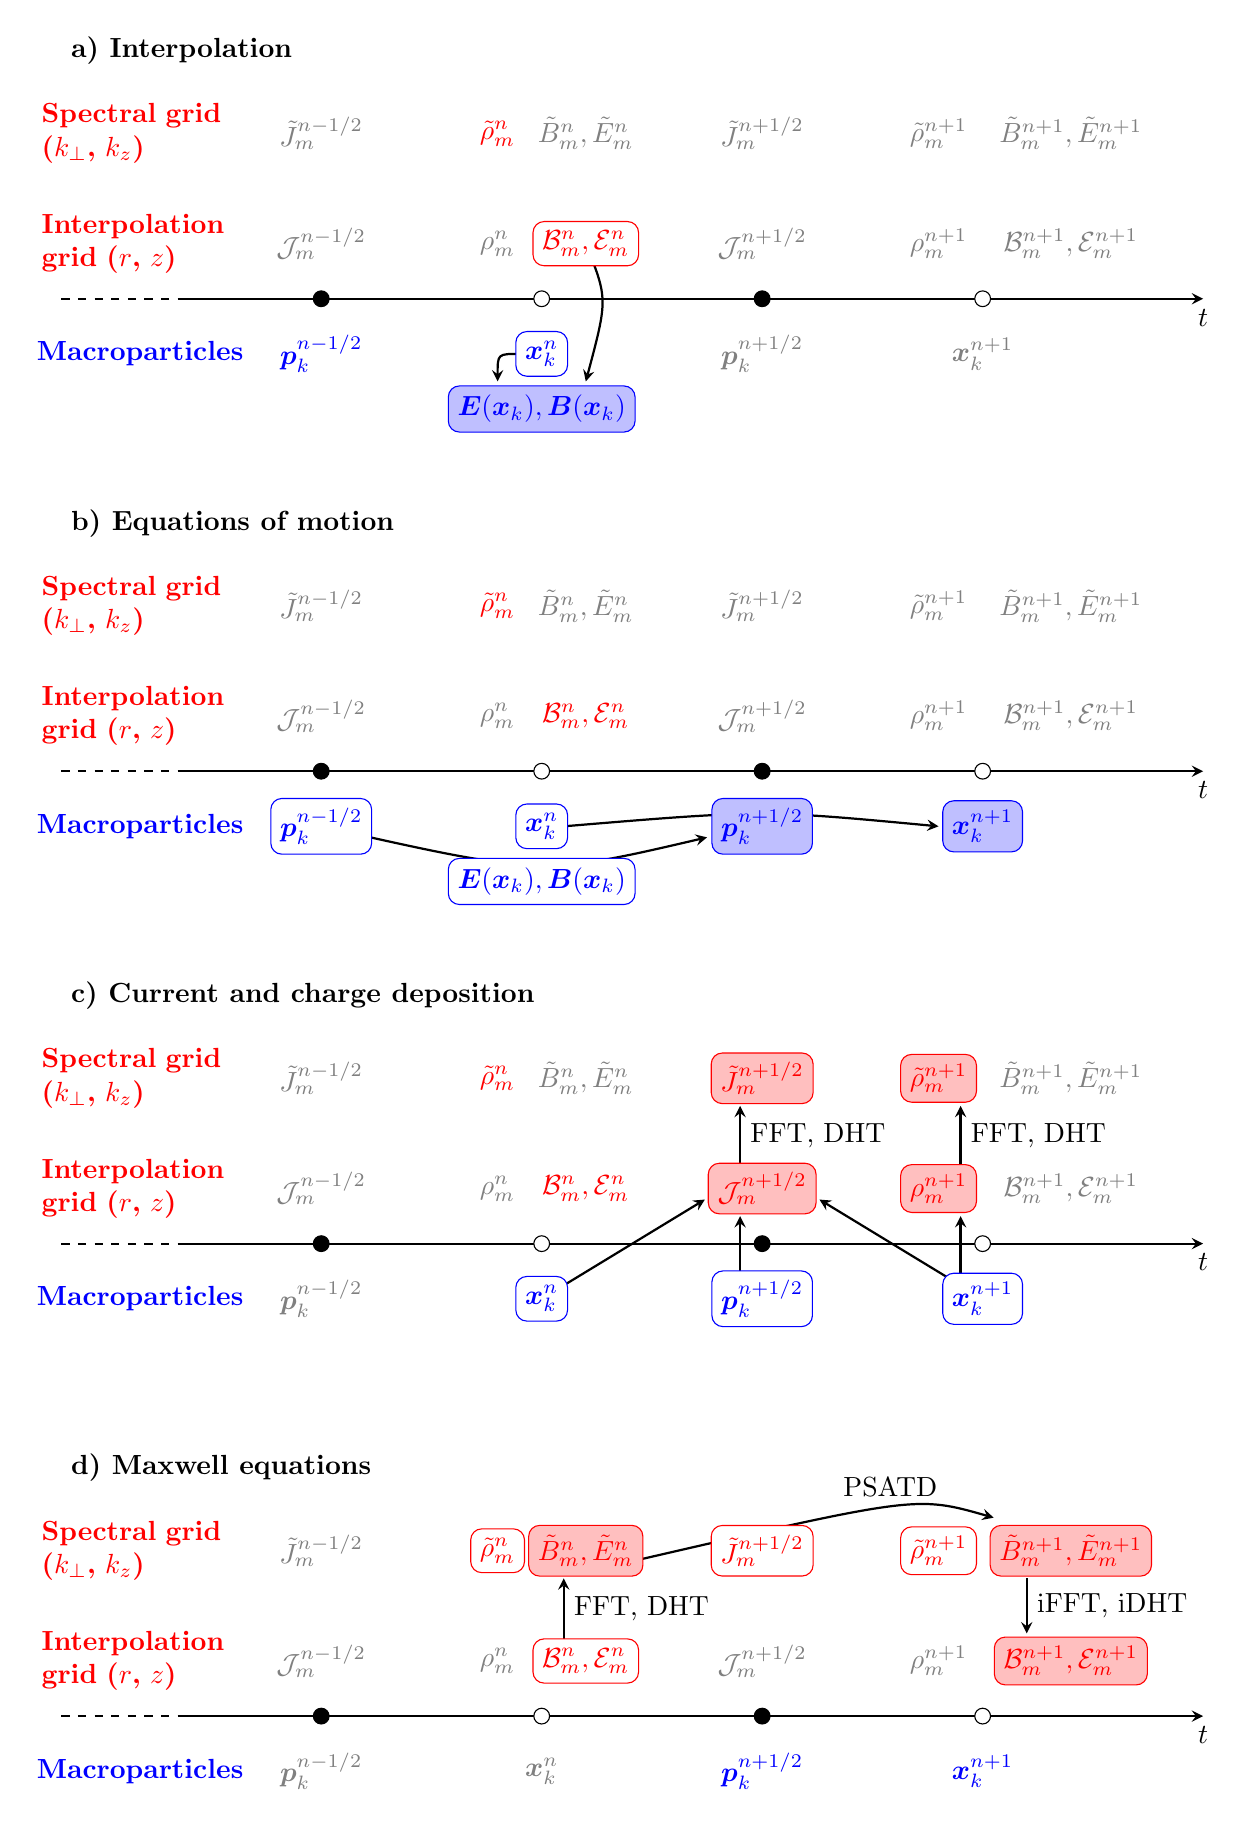
\begin{tikzpicture}
\def \Dt{2.8}
\def \yspac{0.7}

\begin{scope}[yshift=0cm]

\draw (-0.5,4.5*\yspac) node[anchor=west]{\textbf{a) Interpolation}};

% Axes
\draw[thick,->,>=stealth] (1,0) -- (5*\Dt,0) node[below]{$t$};
\draw[thick,dashed] (-0.5,0) -- (1,0);
% Labels
\draw (0.5,3*\yspac) node[red,text width=2.5cm]{\textbf{Spectral grid ($k_\perp$, $k_z$)}};
\draw (0.5,\yspac) node[red,text width=2.5cm]{\textbf{Interpolation grid ($r$, $z$)}};
\draw (0.5,-\yspac) node[blue]{\textbf{Macroparticles}};
% Timesteps
\foreach \n in {1,3} 
\draw[fill=black] (\n*\Dt,0) circle(0.1);
\foreach \n in {2,4} 
\draw[fill=white] (\n*\Dt,0) circle(0.1);
% Arrows
%\draw[->,>=stealth,thick] (3*\Dt,\yspac) -- (2.5*\Dt,-0.25);
%\draw[->,>=stealth,thick] (1.85*\Dt,\yspac) -- (1.85*\Dt,-0.25);
\draw[->,>=stealth,thick] (2.2*\Dt,\yspac) .. controls (2.3*\Dt,0) .. (2.2*\Dt,-1.5*\yspac);
\draw[->,>=stealth,thick] (1.9*\Dt,-1*\yspac) .. controls (1.8*\Dt,-1*\yspac) .. (1.8*\Dt,-1.5*\yspac);
% Fields
% -- n-1/2
\draw (\Dt,3*\yspac) node[gray,fill=white,draw=white,rounded corners]{$ \tilde{J}^{n-1/2}_m$};
\draw (\Dt,1*\yspac) node[gray,fill=white,draw=white,rounded corners]{$ \mathcal{J}^{n-1/2}_m$};
\draw (\Dt,-\yspac) node[blue]{$\vec{p}_k^{n-1/2}$};
% -- n
\draw (1.8*\Dt,3*\yspac) node[red,fill=white,draw=white,rounded corners]{$\tilde{\rho}^n_m$};
\draw (2.2*\Dt,3*\yspac) node[gray,fill=white,draw=white,rounded corners]{$  \tilde{B}^{n}_m, \tilde{E}^{n}_m$};
\draw (1.8*\Dt,\yspac) node[gray,fill=white,draw=white,rounded corners]{$\mathcal{\rho}^n_m$};
\draw (2.2*\Dt,\yspac) node[red,fill=white,draw=red,rounded corners]{$\mathcal{B}^{n}_m, \mathcal{E}^{n}_m$};
\draw (2*\Dt,-\yspac) node[blue,fill=white,draw=blue,rounded corners]{$\vec{x}_k^{n}$};
\draw (2*\Dt,-2*\yspac) node[blue,fill=white!75!blue,draw=blue,rounded corners]{$\vec{E}(\vec{x}_k), \vec{B}(\vec{x}_k)$};
% -- n+1/2
\draw (3*\Dt,3*\yspac) node[gray,fill=white,draw=white,rounded corners]{$ \tilde{J}^{n+1/2}_m$};
\draw (3*\Dt,1*\yspac) node[gray,fill=white,draw=white,rounded corners]{$ \mathcal{J}^{n+1/2}_m$};
\draw (3*\Dt,-\yspac) node[gray]{$\vec{p}_k^{n+1/2}$};
% -- n+1
\draw (3.8*\Dt,3*\yspac) node[gray,fill=white,draw=white,rounded corners]{$\tilde{\rho}^{n+1}_m$};
\draw (4.4*\Dt,3*\yspac) node[gray,fill=white,draw=white,rounded corners]{$  \tilde{B}^{n+1}_m, \tilde{E}^{n+1}_m$};
\draw (3.8*\Dt,\yspac) node[gray,fill=white,draw=white,rounded corners]{$\mathcal{\rho}^{n+1}_m$};
\draw (4.4*\Dt,\yspac) node[gray,fill=white,draw=white,rounded corners]{$\mathcal{B}^{n+1}_m, \mathcal{E}^{n+1}_m$};
\draw (4*\Dt,-\yspac) node[gray]{$\vec{x}_k^{n+1}$};

\end{scope}

\begin{scope}[yshift=-6cm]

\draw (-0.5, 4.5*\yspac) node[anchor=west]{\textbf{b) Equations of motion}};
% Axes
\draw[thick,->,>=stealth] (1,0) -- (5*\Dt,0) node[below]{$t$};
\draw[thick,dashed] (-0.5,0) -- (1,0);
% Labels
\draw (0.5,3*\yspac) node[red,text width=2.5cm]{\textbf{Spectral grid ($k_\perp$, $k_z$)}};
\draw (0.5,\yspac) node[red,text width=2.5cm]{\textbf{Interpolation grid ($r$, $z$)}};
\draw (0.5,-\yspac) node[blue]{\textbf{Macroparticles}};
% Timesteps
\foreach \n in {1,3} 
\draw[fill=black] (\n*\Dt,0) circle(0.1);
\foreach \n in {2,4} 
\draw[fill=white] (\n*\Dt,0) circle(0.1);
% Arrows
%\draw[->,>=stealth,thick] (\Dt,\yspac) -- (1.5*\Dt,-0.25);
%\draw[->,>=stealth,thick] (3*\Dt,\yspac) -- (2.5*\Dt,-0.25);
%\draw[->,>=stealth,thick] (1.85*\Dt,\yspac) -- (1.85*\Dt,-0.25);
\draw[->,>=stealth,thick] (1*\Dt,-\yspac) .. controls (2*\Dt,-1.9*\yspac) .. (2.75*\Dt,-1.2*\yspac);
\draw[->,>=stealth,thick] (2.1*\Dt,-1*\yspac) .. controls (3*\Dt,-0.7*\yspac) .. (3.8*\Dt,-1.*\yspac);
% Fields
% -- n-1/2
\draw (\Dt,3*\yspac) node[gray,fill=white,draw=white,rounded corners]{$ \tilde{J}^{n-1/2}_m$};
\draw (\Dt,1*\yspac) node[gray,fill=white,draw=white,rounded corners]{$ \mathcal{J}^{n-1/2}_m$};
\draw (\Dt,-\yspac) node[blue,fill=white,draw=blue,rounded corners]{$\vec{p}_k^{n-1/2}$};
% -- n
\draw (1.8*\Dt,3*\yspac) node[red,fill=white,draw=white,rounded corners]{$\tilde{\rho}^n_m$};
\draw (2.2*\Dt,3*\yspac) node[gray,fill=white,draw=white,rounded corners]{$  \tilde{B}^{n}_m, \tilde{E}^{n}_m$};
\draw (1.8*\Dt,\yspac) node[gray,fill=white,draw=white,rounded corners]{$\mathcal{\rho}^n_m$};
\draw (2.2*\Dt,\yspac) node[red,fill=white,draw=white,rounded corners]{$\mathcal{B}^n_m, \mathcal{E}^{n}_m$};
\draw (2*\Dt,-\yspac) node[blue,fill=white,draw=blue,rounded corners]{$\vec{x}_k^{n}$};
\draw (2*\Dt,-2*\yspac) node[blue,fill=white,draw=blue,rounded corners]{$\vec{E}(\vec{x}_k), \vec{B}(\vec{x}_k)$};
% -- n+1/2
\draw (3*\Dt,3*\yspac) node[gray,fill=white,draw=white,rounded corners]{$ \tilde{J}^{n+1/2}_m$};
\draw (3*\Dt,1*\yspac) node[gray,fill=white,draw=white,rounded corners]{$ \mathcal{J}^{n+1/2}_m$};
\draw (3*\Dt,-\yspac) node[blue,fill=white!75!blue,draw=blue,rounded corners]{$\vec{p}_k^{n+1/2}$};
% -- n+1
\draw (3.8*\Dt,3*\yspac) node[gray,fill=white,draw=white,rounded corners]{$\tilde{\rho}^{n+1}_m$};
\draw (4.4*\Dt,3*\yspac) node[gray,fill=white,draw=white,rounded corners]{$  \tilde{B}^{n+1}_m, \tilde{E}^{n+1}_m$};
\draw (3.8*\Dt,\yspac) node[gray,fill=white,draw=white,rounded corners]{$\mathcal{\rho}^{n+1}_m$};
\draw (4.4*\Dt,\yspac) node[gray,fill=white,draw=white,rounded corners]{$\mathcal{B}^{n+1}_m, \mathcal{E}^{n+1}_m$};
\draw (4*\Dt,-\yspac) node[blue,fill=white!75!blue,draw=blue,rounded corners]{$\vec{x}_k^{n+1}$};

\end{scope}

\begin{scope}[yshift=-12cm]

\draw (-0.5,4.5*\yspac) node[anchor=west]{\textbf{c) Current and charge deposition}};

% Axes
\draw[thick,->,>=stealth] (1,0) -- (5*\Dt,0) node[below]{$t$};
\draw[thick,dashed] (-0.5,0) -- (1,0);
% Labels
\draw (0.5,3*\yspac) node[red,text width=2.5cm]{\textbf{Spectral grid ($k_\perp$, $k_z$)}};
\draw (0.5,\yspac) node[red,text width=2.5cm]{\textbf{Interpolation grid ($r$, $z$)}};
\draw (0.5,-\yspac) node[blue]{\textbf{Macroparticles}};
% Timesteps
\foreach \n in {1,3} 
\draw[fill=black] (\n*\Dt,0) circle(0.1);
\foreach \n in {2,4} 
\draw[fill=white] (\n*\Dt,0) circle(0.1);
% Arrows
\draw[->,>=stealth,thick] (2*\Dt,-\yspac) -- (2.74*\Dt,0.8*\yspac);
\draw[->,>=stealth,thick] (2.9*\Dt,-\yspac) -- (2.9*\Dt,0.5*\yspac);
\draw[->,>=stealth,thick] (2.9*\Dt,1.4*\yspac) -- node[anchor=west]{FFT, DHT}(2.9*\Dt,2.5*\yspac);
\draw[->,>=stealth,thick] (4*\Dt,-\yspac) -- (3.26*\Dt,0.8*\yspac);
\draw[->,>=stealth,thick] (3.9*\Dt,-\yspac) -- (3.9*\Dt,0.5*\yspac);
\draw[->,>=stealth,thick] (3.9*\Dt,1.4*\yspac) -- node[anchor=west]{FFT, DHT}(3.9*\Dt,2.5*\yspac);
%\draw[->,>=stealth,thick] (3*\Dt,\yspac) -- (2.5*\Dt,-0.25);
%\draw[->,>=stealth,thick] (1.85*\Dt,\yspac) -- (1.85*\Dt,-0.25);
%\draw[->,>=stealth,thick] (1*\Dt,-\yspac) .. controls (2*\Dt,-1.9*\yspac) .. (2.75*\Dt,-1.2*\yspac);
%\draw[->,>=stealth,thick] (2.1*\Dt,-1*\yspac) .. controls (3*\Dt,-0.7*\yspac) .. (3.8*\Dt,-1.*\yspac);
% Fields
% -- n-1/2
\draw (\Dt,3*\yspac) node[gray,fill=white,draw=white,rounded corners]{$ \tilde{J}^{n-1/2}_m$};
\draw (\Dt,1*\yspac) node[gray,fill=white,draw=white,rounded corners]{$ \mathcal{J}^{n-1/2}_m$};
\draw (\Dt,-\yspac) node[gray,fill=white,draw=white,rounded corners]{$\vec{p}_k^{n-1/2}$};
% -- n
\draw (1.8*\Dt,3*\yspac) node[red,fill=white,draw=white,rounded corners]{$\tilde{\rho}^n_m$};
\draw (2.2*\Dt,3*\yspac) node[gray,fill=white,draw=white,rounded corners]{$  \tilde{B}^{n}_m, \tilde{E}^{n}_m$};
\draw (1.8*\Dt,\yspac) node[gray,fill=white,draw=white,rounded corners]{$\mathcal{\rho}^n_m$};
\draw (2.2*\Dt,\yspac) node[red,fill=white,draw=white,rounded corners]{$\mathcal{B}^n_m, \mathcal{E}^{n}_m$};
\draw (2*\Dt,-\yspac) node[blue,fill=white,draw=blue,rounded corners]{$\vec{x}_k^{n}$};
% -- n+1/2
\draw (3*\Dt,3*\yspac) node[red,fill=white!75!red,draw=red,rounded corners]{$ \tilde{J}^{n+1/2}_m$};
\draw (3*\Dt,1*\yspac) node[red,fill=white!75!red,draw=red,rounded corners]{$ \mathcal{J}^{n+1/2}_m$};
\draw (3*\Dt,-\yspac) node[blue,fill=white,draw=blue,rounded corners]{$\vec{p}_k^{n+1/2}$};
% -- n+1
\draw (3.8*\Dt,3*\yspac) node[red,fill=white!75!red,draw=red,rounded corners]{$\tilde{\rho}^{n+1}_m$};
\draw (4.4*\Dt,3*\yspac) node[gray,fill=white,draw=white,rounded corners]{$  \tilde{B}^{n+1}_m, \tilde{E}^{n+1}_m$};
\draw (3.8*\Dt,\yspac) node[red,fill=white!75!red,draw=red,rounded corners]{$\mathcal{\rho}^{n+1}_m$};
\draw (4.4*\Dt,\yspac) node[gray,fill=white,draw=white,rounded corners]{$\mathcal{B}^{n+1}_m, \mathcal{E}^{n+1}_m$};
\draw (4*\Dt,-\yspac) node[blue,fill=white,draw=blue,rounded corners]{$\vec{x}_k^{n+1}$};

\end{scope}

\begin{scope}[yshift=-18cm]

\draw (-0.5,4.5*\yspac) node[anchor=west]{\textbf{d) Maxwell equations}};

% Axes
\draw[thick,->,>=stealth] (1,0) -- (5*\Dt,0) node[below]{$t$};
\draw[thick,dashed] (-0.5,0) -- (1,0);
% Labels
\draw (0.5,3*\yspac) node[red,text width=2.5cm]{\textbf{Spectral grid ($k_\perp$, $k_z$)}};
\draw (0.5,\yspac) node[red,text width=2.5cm]{\textbf{Interpolation grid ($r$, $z$)}};
\draw (0.5,-\yspac) node[blue]{\textbf{Macroparticles}};
% Timesteps
\foreach \n in {1,3} 
\draw[fill=black] (\n*\Dt,0) circle(0.1);
\foreach \n in {2,4} 
\draw[fill=white] (\n*\Dt,0) circle(0.1);
% Arrows
%\draw[->,>=stealth,thick] (2*\Dt,-\yspac) -- (2.74*\Dt,0.8*\yspac);
%\draw[->,>=stealth,thick] (2.9*\Dt,-\yspac) -- (2.9*\Dt,0.5*\yspac);
\draw[->,>=stealth,thick] (2.1*\Dt,1.4*\yspac) -- node[anchor=west]{FFT, DHT}(2.1*\Dt,2.5*\yspac);
%\draw[->,>=stealth,thick] (4*\Dt,-\yspac) -- (3.26*\Dt,0.8*\yspac);
%\draw[->,>=stealth,thick] (3.9*\Dt,-\yspac) -- (3.9*\Dt,0.5*\yspac);
\draw[<-,>=stealth,thick] (4.2*\Dt,1.5*\yspac) -- node[anchor=west]{iFFT, iDHT}(4.2*\Dt,2.5*\yspac);
%\draw[->,>=stealth,thick] (3*\Dt,\yspac) -- (2.5*\Dt,-0.25);
%\draw[->,>=stealth,thick] (1.85*\Dt,\yspac) -- (1.85*\Dt,-0.25);
%\draw[->,>=stealth,thick] (1*\Dt,-\yspac) .. controls (2*\Dt,-1.9*\yspac) .. (2.75*\Dt,-1.2*\yspac);
\draw[->,>=stealth,thick] (2.4*\Dt,2.8*\yspac) .. controls (3.7*\Dt,4*\yspac) .. node[above]{PSATD} (4.05*\Dt,3.6*\yspac);
% Fields
% -- n-1/2
\draw (\Dt,3*\yspac) node[gray,fill=white,draw=white,rounded corners]{$ \tilde{J}^{n-1/2}_m$};
\draw (\Dt,1*\yspac) node[gray,fill=white,draw=white,rounded corners]{$ \mathcal{J}^{n-1/2}_m$};
\draw (\Dt,-\yspac) node[gray,fill=white,draw=white,rounded corners]{$\vec{p}_k^{n-1/2}$};
% -- n
\draw (1.8*\Dt,3*\yspac) node[red,fill=white,draw=red,rounded corners]{$\tilde{\rho}^n_m$};
\draw (2.2*\Dt,3*\yspac) node[red,fill=white!75!red,draw=red,rounded corners]{$  \tilde{B}^{n}_m, \tilde{E}^{n}_m$};
\draw (1.8*\Dt,\yspac) node[gray,fill=white,draw=white,rounded corners]{$\mathcal{\rho}^n_m$};
\draw (2.2*\Dt,\yspac) node[red,fill=white,draw=red,rounded corners]{$\mathcal{B}^n_m, \mathcal{E}^{n}_m$};
\draw (2*\Dt,-\yspac) node[gray]{$\vec{x}_k^{n}$};
% -- n+1/2
\draw (3*\Dt,3*\yspac) node[red,fill=white,draw=red,rounded corners]{$ \tilde{J}^{n+1/2}_m$};
\draw (3*\Dt,1*\yspac) node[gray,fill=white,draw=white,rounded corners]{$ \mathcal{J}^{n+1/2}_m$};
\draw (3*\Dt,-\yspac) node[blue]{$\vec{p}_k^{n+1/2}$};
% -- n+1
\draw (3.8*\Dt,3*\yspac) node[red,fill=white,draw=red,rounded corners]{$\tilde{\rho}^{n+1}_m$};
\draw (4.4*\Dt,3*\yspac) node[red,fill=white!75!red,draw=red,rounded corners]{$  \tilde{B}^{n+1}_m, \tilde{E}^{n+1}_m$};
\draw (3.8*\Dt,\yspac) node[gray,fill=white,draw=white,rounded corners]{$\mathcal{\rho}^{n+1}_m$};
\draw (4.4*\Dt,\yspac) node[red,fill=white!75!red,draw=red,rounded corners]{$\mathcal{B}^{n+1}_m, \mathcal{E}^{n+1}_m$};
\draw (4*\Dt,-\yspac) node[blue]{$\vec{x}_k^{n+1}$};

\end{scope}

\end{tikzpicture}


\caption{\label{fig:GlobalScheme}Schematic description of the 4 steps
  of a PIC
  cycle. At any given time, the quantities that
  are known are shown in color (red and blue), 
while the quantities that are unknown or have been erased from memory 
are shown in gray. The quantities that are being calculated at a given step are
  displayed with a colored background, and arrows indicate which
  quantities are used for this calculation.}
\end{figure}


\subsection{Transverse discretization of the intermediate grid, 
of the spectral grid and of the Hankel Transform}
\label{sec:discretization}

When transforming from the intermediate to the spectral grid, the FFT
algorithm is the natural way to discretize the Fourier transform along $z$, due to its
favorable computational scaling ($\propto N_z\log(N_z)$).
On the other hand, there are a variety of existing algorithms (that are not mathematically
equivalent) to discretize the Hankel
transform (e.g. \citep{Cree,Yu,Siegman,Guizar,KaiMing}), and the use of one or the other
is very dependent on the pursued application. Broadly
speaking, chosing an algorithm for the Discrete Hankel Transform (DHT)
algorithms consists in 
\begin{itemize}
\item Choosing a discrete grid in $r$ and $k_\perp$ space, on which to
  sample the functions to be transformed. In some algorithms, these
  grids may not be evenly-spaced, and can be for instance
  logarithmically spaced \citep{Siegman} or correspond to the zeros of
  Bessel functions \citep{Yu,Guizar,KaiMing}.
\item Once a grid is chosen, the DHT amounts to a linear operation on a
  finite set of points (the points of the grid) and can thus be
  represented by a matrix. Thus the second choice is that of a matrix
  that represents, as closely as possible, the exact Hankel Transform.
\end{itemize}
Here, we choose to discretize the algorithm on an evenly-spaced grid in $r$
(for the intermediate grid) :
\[ r_j = \Delta r \left( j+\frac{1}{2} \right) \qquad  j \in \{0, ...,
N_r-1 \} \qquad \mathrm{where} \quad \Delta r = \frac{r_{max}}{N_r} \]
but on an irregular grid in $k_\perp$ (for the spectral grid). This is because the authorized
$k_\perp$ are determined by the boundary conditions, in the same way that
the periodic boundaries in a Cartesian code impose the use of
evenly-spaced $k$. Here, for simplicity, we impose that the
longitudinal fields be $0$ at $r_{max}$ (i.e. $E_z(r_{max}, z) = 0$,
$B_z(r_{max}, z) = 0$). In this case, it turns out that the set of authorized
$k_\perp$ depends on the azimuthal mode $m$ and reads
\[  k^m_{\perp,j} = \frac{\alpha_j^m}{r_{max}} \qquad j \in \{0, ..., N_r-1 \}\]
where $\alpha^m_j$ is the $j$th positive zero of the Bessel function of order
$m$ $J_m$ (including the trivial value $\alpha_0^m=0$ for
$m>0$). These values are represented in figure \ref{fig:Kgrid}. Notice
that it is not an issue that the spectral components $\spectral{F}_m$
for different azimuthal modes $m$ are discretized on different
$k_\perp$ grids, since each azimuthal mode $m$ evolves separately in
\cref{eq:CircMaxwellp,eq:CircMaxwellm,eq:CircMaxwellz}.

\begin{figure}[!h]
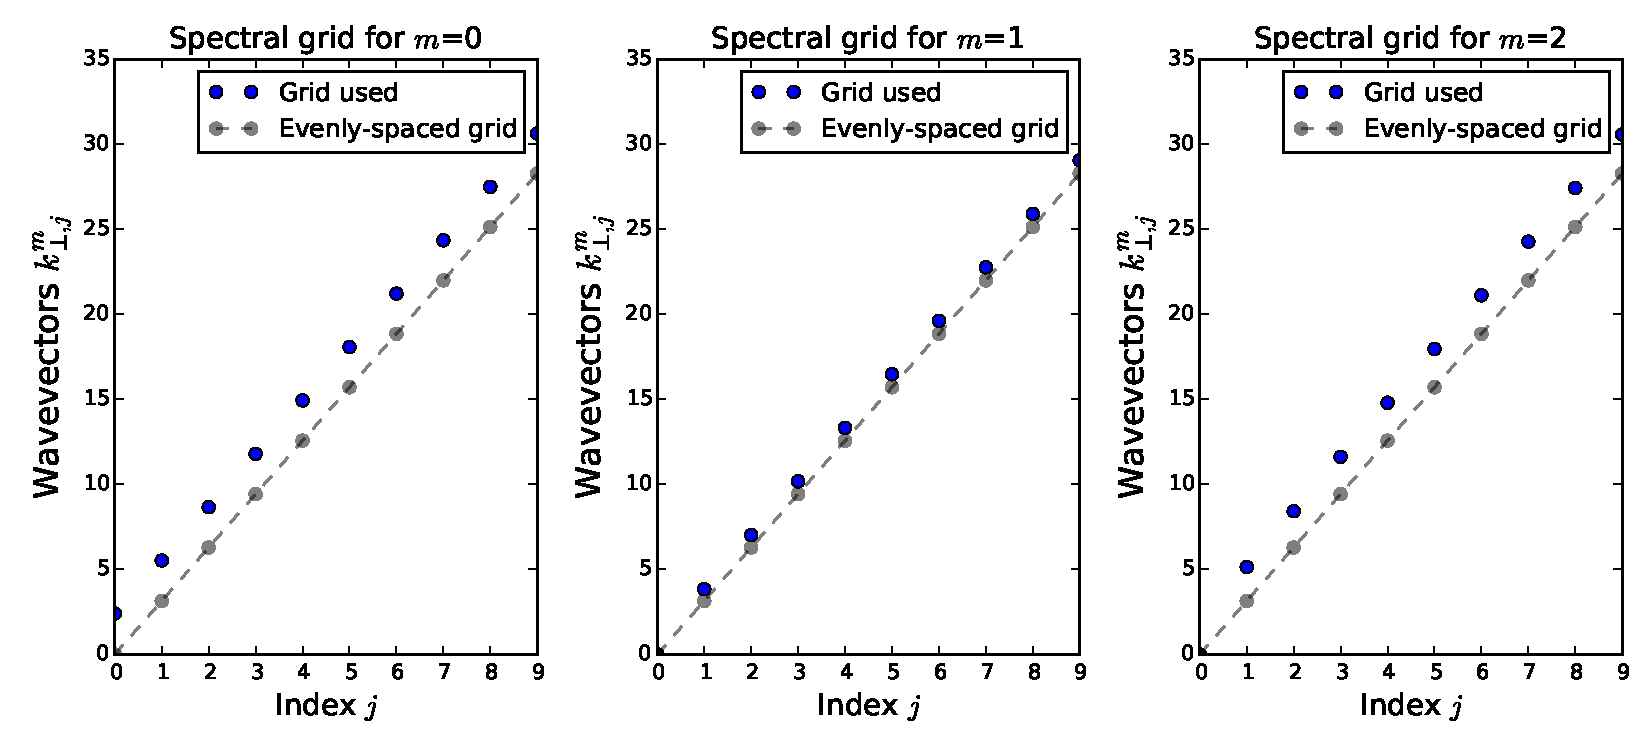
\includegraphics[width=\textwidth]{figures/KGrid.pdf}
\caption{\label{fig:Kgrid}Position of the grid points in $k_\perp$ space
  (blue dots) for the azimuthal modes $m=0$, $m=1$ and $m=2$ for $N_r
  = 10$ and $r_{max}=1$. These values are compared with those of an
  evenly-spaced grid used in spectral Cartesian codes (grey dots, $k_j = j\pi/r_{max}$).}
\end{figure}

As mentioned above, once this grid is set up, the Discrete Hankel Transform is simply a
linear operation on a finite set of points, and can thus be
represented by a matrix operation.
\[ \mathrm{DHT^m_n}[f] \,(k^m_{\perp,j}) = \sum_{p=0}^{N_r-1} (M_{n,m})_{j,p}
\;f(r_p) \qquad \mathrm{IDHT^m_n}[g] \, (r_j) = \sum_{p=0}^{N_r-1}
(M'_{n,m})_{j,p} \; g(k^m_{\perp,p}) \]

Notice that the $N_r\times N_r$ transformation matrices $M_{n,m}$ and
$M_{n,m}'$ depend on $n$ (order of the Hankel transform) and $m$
(index of the azimuthal mode, and thus index of the spectral grid
$k^m_{\perp,j}$ on which the Hankel transform is performed). 
In practice, $n$ and $m$ are either equal or they differ by
$\pm 1$ (e.g. in \cref{eq:FTHTr,eq:FTHTt}, when the azimuthal mode $m$ is
transformed using the Hankel transform of order $m+1$ or $m-1$.)

The expressions of $M_{n,m}$ and $M'_{n,m}$, for the DHT algorithm
that we chose, are given in \ref{sec:HTMatrix}. 
%This particular choice is very specific and
%dependent on the imposed boundary conditions at $r_{max}$ ; in future
%work, different implementations of the DHT could be used depending on
%the boundary conditions. 
In practice,  these matrices need to be
computed only once (at the beginning of the simulation) and can then be used at each
iteration. Notice also that the computational time for this
matrix multiplication is proportional to $N_r^2$, which is slow
compared to a 1D FFT ($\propto N_r \log(N_r)$), but
still faster than the 2D FFT ($\propto N_x N_y \log(N_x) + N_x N_y \log(N_y) $)
which is typically used in a spectral 3D Cartesian code. 


\subsection{Field gathering}

When gathering the fields from the intermediate grid to the
macroparticles (see \cref{fig:GlobalScheme}),
we use the standard linear shape factors :
\begin{align} 
F_u(\vec{r}_k) &=  \sum_{p,q} S_{z,p}(z_k)S_{r,q}(r_k) \left[ \sum_{m=-N_m}^{N_m} \hat{F}_{u,m}(z_p, r_q)
  e^{-im\theta_k} \right] \\
& = \sum_{p,q} S_{z,p}(z_k)S_{r,q}(r_k) \left[ \hat{F}_{u,0}(z_p,
  r_q) + 2\,\Re \left( \sum_{m=1}^{N_m} \hat{F}_{u,m}(z_p, r_q)
  e^{-im\theta_k} \right) \right] \label{eq:gathering}
\end{align}
where $F$ is either $E$ or $B$, $u$ is either $r$, $\theta$ or $z$, $k$ is the index of the macroparticle,
and $p$ and $q$ are the indices of the two nearest cells in $z$ and
$r$ respectively. $N_m$ is the total number
of azimuthal modes used. Notice that, in \cref{eq:gathering}, we used the fact that
$\hat{F}_{u,-m}(z,r) = \hat{F}^*_{u,m}(z,r) $, which can be
inferred from \cref{eq:IntermFwTrans}. Incidentally, \cref{eq:gathering} shows that only the modes
with $m\geq 0$ need to be taken into account in the code, as they are 
sufficient to retrieve the force on the macroparticles.

Finally, in \cref{eq:gathering}, $S_{z,p}$ and $S_{z,q}$ are the linear
shape factors in $z$ and $r$ :
\[ S_{z,p_0}(z) = \frac{z_{p_0+1}- z}{\Delta z}  \qquad 
S_{z,p_0 +1}(z) = \frac{ z - z_{p_0} }{\Delta z} \qquad
\mathrm{with} \quad z_{p_0} \leq z < z_{p_0 +1}  \]
\[ S_{r,q_0}(r) = \frac{ r_{q_0+1} - r }{  \Delta r }
\qquad S_{r,q_0+1}(r) = \frac{ r - r_{q_0} }{  \Delta r }
\qquad \mathrm{with} \quad r_{q_0} \leq r < r_{q_0+1}
 \]
%\noindent Additionally, for particles that are located in the first half of the first
%cell ($0< r < \Delta r/2$), the shape $S_{r,0}$ is modified and reads
%\[ S_{r,0}(r) = \frac{2r}{\Delta r} \]
%\noindent This expression is chosen so as to ensure that a uniform particle
%distribution yields a uniform charge density, even on the axis. (This
%is a common issue for quasi-cylindrical algorithms, and is discussed e.g. in
%\citep{Verboncoeur}).

\subsection{Equations of motion}

Since the macroparticles are evolved in 3D, we compute
the Cartesian components $E_x$, $E_y$, $E_z$, $B_x$, $B_y$ and
$B_z$, from the fields $E_r$, $E_\theta$, $E_z$, $B_r$, $B_\theta$ and
$B_z$ that were gathered at the positions of each macroparticle. 
We then advance the equations of motion
\[ \frac{d\vec{p}}{dt} = q\vec{E} + q\vec{v}\times \vec{B} \qquad
\frac{d\vec{x}}{dt} = \frac{\vec{p}}{\gamma \,m} \]
\noindent  in standard 3D Cartesian coordinates, by using the leap-frog pusher described in \citep{VayPoP2008}.

\subsection{Current deposition}
\label{sec:current-deposition}

As in \citep{Lifschitz}, the charge density is calculated on the intermediate grid in the
following way:
\[ \hat{\rho}_m(z_p,r_q) = \frac{ \sum_k  S_{z,p}(z_k)S_{r,q}(r_k) Q_k e^{im\theta_k}}{V_{q}} \]
where $Q_k$ is the charge of the macroparticle with index $k$, and
where $V_q$ is the volume of a cell, which is for our grid
\[ V_{q} = \pi [\, (q+1)^2- q^2\,] \Delta r^2 \Delta z \]

\noindent Similarly, the current deposition is given by
\[ \hat{j}_{u,m}(z_p,r_q) = \frac{\sum_k S_{z,p}(z_k) S_{r,q}(r_k)
Q_k v_{u,k} e^{im\theta_k}}{V_{q}} \]
where $u = z,r,\theta$ and the $v_{u,k}$ are the cylindrical components of the
velocity of the macroparticle $k$. As mentioned previously, once the
macroparticles have deposited their charge and current on the
intermediate grid, we transform them to the spectral grid, using an
FFT and a DHT (see \cref{fig:GlobalScheme}).

Smoothing is then typically applied on the charge and currents, after they
have been deposited to the grid (but no smoothing is applied on the
fields $E$ and $B$ directly). This is done so as to avoid the accumulation
of noise at high frequency, in the simulations. This smoothing
is performed directly in spectral space, by multiplying the charge
and currents by a transfer function $\spectral{T}(k_z, k_\perp)$ which, 
in a 2D Cartesian algorithm, 
would be equivalent to a single-pass binomial filter \citep{Birdsall2004}.
\[ \spectral{T}(k_z, k_r) = \cos^2 \left( \frac{k_z}{k_{z,max}}\frac{\pi}{2} \right)
\cos^2\left( \frac{k_\perp}{k_{\perp,max}}\frac{\pi}{2} \right) \]
\noindent where $k_{z, max}$ and $k_{\perp,max}$ are the highest
wavevectors that the discrete spectral grid supports, in the
longitudinal and transverse direction.

Notice also that, in the above deposition scheme, we do not attempt to
reproduce the Esirkepov current deposition \citep{Esirkepov}, and instead use a
simple direct current deposition. It is well-known that this simple deposition does not necessarily
satisfy the relation $\partial_t\rho + \vec{\nabla}\cdot\vec{j} =
0$, but that this can be corrected for, by slightly modifying the
currents without modifying their curl:
\[ \vec{j}' = \vec{j} - \vec{\nabla} G \]
where $G$ satisfies the Poisson-like equation
\[ \vec{\nabla}^2 G = \partial_t\rho + \vec{\nabla}\cdot\vec{j} \]

The above equation is typically expensive to solve on a spatial grid, but
very easy to solve in spectral space. In spectral space and with the
notations of \cref{fig:GlobalScheme}, these equations become
\[ \spectral{J}'^{n+1/2}_{+,m} = \spectral{J}^{n+1/2}_{+,m} +
\frac{k_\perp}{2} \spectral{G}^{n+1/2}_m
\qquad
\spectral{J}'^{n+1/2}_{-,m} = \spectral{J}^{n+1/2}_{-,m} - \frac{k_\perp}{2} \spectral{G}^{n+1/2}_m
\qquad \spectral{J}'^{n+1/2}_{z,m} = \spectral{J}^{n+1/2}_{z,m} - ik_z
\spectral{G}^{n+1/2}_m\]
with
\[ \spectral{G}^{n+1/2}_m = - \frac{1}{k_\perp^2 + k_z^2}\left(
  \frac{\spectral{\rho}^{n+1}_m -\spectral{\rho}^{n}_m}{\Delta t} + k_\perp
  (\spectral{J}^{n+1/2}_{+,m} -\spectral{J}^{n+1/2}_{-,m}) + ik_z\spectral{J}^{n+1/2}_{z,m}  \right) \]
With this correction, the new currents $\spectral{J}'^{n+1/2}$ do satisfy
the charge conservation equation \cref{eq:SpectCharge}. Therefore we apply this
correction in spectral space, at the end of the current deposition at each timestep.

\subsection{Integration of the Maxwell equation using the PSATD scheme}
\label{sec:FieldIntegration}

The Maxwell equations
\cref{eq:CircMaxwellp,eq:CircMaxwellm,eq:CircMaxwellz} could in
principle be integrated in time by using a finite difference scheme:
\begin{align*}
\tE{+}{n+1} = \; & \tE{+}{n} + 
c^2\Delta t\left(-\frac{ik_\perp }{2} \tB{z}{n} + k_z\tB{+}{n}
- \mu_0 \tj{+}{n+1/2} \right) & \\
\tE{-}{n+1} =\; & \tE{-}{n} +
c^2\Delta t\left(- \frac{ik_\perp }{2} \tB{z}{n} - k_z\tB{-}{n}
- \mu_0 \tj{-}{n+1/2} \right) &\\
\tE{z}{n+1} =\; & \tE{z}{n} + 
c^2\Delta t\left(ik_\perp \tB{+}{n} + ik_\perp \tB{-}{n}
- \mu_0 \tj{z}{n+1/2} \right)  &
\end{align*}
\begin{align*}
\tB{+}{n+1} = \; & \tB{+}{n} - 
\Delta t\left(-\frac{ik_\perp }{2} \tE{z}{n} + k_z\tE{+}{n}
\right) & \\
\tB{-}{n+1} =\; & \tB{-}{n} - 
\Delta t\left(- \frac{ik_\perp }{2} \tE{z}{n} - k_z\tE{-}{n}
\right) &\\
\tB{z}{n+1} =\; & \tB{z}{n} - 
\Delta t\left(ik_\perp \tE{+}{n} + ik_\perp \tE{-}{n}
\right) &
\end{align*}
However, this type of scheme retains some amount of numerical dispersion, and can
thus affect the simulated physics.

Instead, here we use an adaptation of the PSATD scheme \citep{Haber} for the
Fourier-Bessel spectral space. As in the case of the standard
PSATD, we assume that the currents are constant over one timestep and
that the charge density is linear in time over the same timestep. Under these
assumptions, the Maxwell equations \cref{eq:CircMaxwellp,eq:CircMaxwellm,eq:CircMaxwellz} can be integrated
analytically over that timestep, and they lead to:
\begin{align*}
\tE{+}{n+1} = \; & C \tE{+}{n} + 
c^2\frac{S}{\omega}\left(-\frac{ik_\perp }{2} \tB{z}{n} + k_z\tB{+}{n}
- \mu_0 \tj{+}{n+1/2} \right) + \frac{c^2}{\epsilon_0}
\frac{k_\perp}{2}\left[ \frac{\trho{n+1}}{\omega^2}\left(
  1 - \frac{S}{\omega\Delta t}\right) -
\frac{\trho{n}}{\omega^2}\left( C -\frac{S}{\omega\Delta t}\right)\right]  & \\
\tE{-}{n+1} =\; & C \tE{-}{n} +
c^2\frac{S}{\omega}\left(- \frac{ik_\perp }{2} \tB{z}{n} - k_z\tB{-}{n}
- \mu_0 \tj{-}{n+1/2} \right) - \frac{c^2}{\epsilon_0}
\frac{k_\perp}{2}\left[ \frac{\trho{n+1}}{\omega^2}\left(
  1 - \frac{S}{\omega\Delta t}\right) - \frac{\trho{n}}{\omega^2}
\left( C - \frac{S}{\omega\Delta t}\right)\right]  &\\
\tE{z}{n+1} =\; & C \tE{z}{n} + 
c^2\frac{S}{\omega}\left(ik_\perp \tB{+}{n} + ik_\perp \tB{-}{n}
- \mu_0 \tj{z}{n+1/2} \right) - \frac{c^2}{\epsilon_0}
ik_z\left[ \frac{\trho{n+1}}{\omega^2}\left(
  1 - \frac{S}{\omega\Delta t}\right) - \frac{\trho{n}}{\omega^2}
\left( C - \frac{S}{\omega\Delta t}\right)\right]  &
\end{align*}
\begin{align*}
\tB{+}{n+1} = \; & C \tB{+}{n} - 
\frac{S}{\omega}\left(-\frac{ik_\perp }{2} \tE{z}{n} + k_z\tE{+}{n}
\right) + \mu_0 c^2\frac{1-C}{\omega^2} \left( -\frac{ik_\perp }{2}
  \tj{z}{n+1/2} + k_z \tj{+}{n+1/2} \right)& \\
\tB{-}{n+1} =\; & C \tB{-}{n} - 
\frac{S}{\omega}\left(- \frac{ik_\perp }{2} \tE{z}{n} - k_z\tE{-}{n}
\right) + \mu_0 c^2\frac{1-C}{\omega^2} \left( - \frac{ik_\perp }{2}
  \tj{z}{n+1/2} - k_z \tj{-}{n+1/2} \right) &\\
\tB{z}{n+1} =\; & C \tB{z}{n} - 
\frac{S}{\omega}\left(ik_\perp \tE{+}{n} + ik_\perp \tE{-}{n}
\right) + \mu_0 c^2\frac{1-C}{\omega^2} \left( ik_\perp
  \tj{+}{n+1/2} + ik_\perp \tj{-}{n+1/2} \right)&
\end{align*}

\noindent where $\omega \equiv c\sqrt{k_z^2 + k_\perp^2}$, $C \equiv \cos(\omega \Delta t)$
and $S \equiv \sin(\omega \Delta t) $. (See \ref{sec:PSTADderiv} for a
derivation of these equations.)

\subsection{Practical implementation}

The full PIC algorithm described in this section was implemented in a
code written in Python. For performance, this implementation makes use of the
pre-compiled libraries FFTW and BLAS (for the matrix multiplication
  in the DHT), and utilizes the Numba just-in-time compiler for the
  computationally-intensive parts of the code. In addition, the code
  was developed for both single-CPU and single-GPU architectures (with the GPU runs
  being typically more than 40 times faster than the equivalent CPU runs, on
  modern hardware). A multi-CPU/multi-GPU version will be developed in
  the future.

\section{Benchmarks}
\label{sec:benchmarks}

We tested the above algorithm in a number of physical situations. In
particular, we emphasize here the tests of the dispersion relation, since the absence of
spurious numerical dispersion was one of the original goals of this algorithm.

\subsection{Propagation in vacuum}
\label{sec:vacuum_vg}

A first test consisted in letting a laser pulse propagate in vacuum and in
measuring its group velocity in the simulation. These simulations were
run with the spectral quasi-cylindrical algorithm presented in
\cref{sec:implementation}, but also, for comparison, with a finite-difference quasi-cylindrical
algorithm equivalent to that of \cite{Lifschitz,Davidson} and which had
been previously implemented in the PIC code \textsc{Warp}.

The simulations were run with a moving window, in a box with a
longitudinal size of 40 $\mu$m and a transverse size of 48 $\mu$m. (In
the case of the spectral algorithm, the fields were damped at the back
of the moving window, in a similar way as in \citep{YuIPAC2015}.)
The laser pulse itself was initialized at focus, with a waist 
$w_0 = 16 \;\mathrm{\mu m}$, a length $L = 10 \; \mathrm{\mu m}$,
a wavelength $\lambda = 0.8 \; \mathrm{\mu m}$ and a 
dimensionless potential vector $a_0 = 10^{-2}$.
The resolution was varied while keeping the same cell aspect ratio ($\Delta r = 5\Delta z$). The
timestep was set to $c\Delta t = \Delta z$ in the case of the spectral
quasi-cylindrical algorithm and to $c\Delta t = 1/\sqrt{1/\Delta z^2 +
  2/\Delta r^2}$ in the case of the finite-difference
quasi-cylindrical algorithm (due to the existence of a Courant
limit for this algorithm). 

Physically, the on-axis group velocity of the pulse should be slightly lower than $c$ due
to the finite waist of the pulse (see e.g. \citep{Esarey1999}). The
analytical expression for the corresponding relative
difference in on-axis group velocity is
\begin{equation} 
\label{eq:vacuum_vg}
\frac{c-v_g}{c} = 2\left( \frac{\lambda}{2\pi w_0} \right)^2
\end{equation}
\noindent In the case at hand ($w_0=16\;\mathrm{\mu m}$,
$\lambda=0.8\;\mathrm{\mu m}$), this relative difference is extremely
small ($(c-v_g)/c = 1.27 \times 10^{-4}$), and it may be difficult for
PIC codes to capture this small physical difference. 

To assess the capacities of the finite-difference and
spectral quasi-cylindrical code in this regard, \cref{fig:Vacuum_vg} displays the relative
difference in group velocity, as measured in the
simulations. As can be expected, in the
finite-difference simulations, the
group velocity of the laser depends on the resolution, due to numerical
dispersion. 
Moreover, this group velocity is considerably different than the analytical
prediction, even for a relatively high resolution (40 gridpoints per
wavelength). On the other hand, with the spectral algorithm described
here, the group velocity is practically independent of the resolution, and
displays very good agreement with the analytical prediction. 
This corroborates the fact that the spectral quasi-cylindrical algorithm
described here has no numerical dispersion in vacuum.

\begin{figure}[!h]
\centering
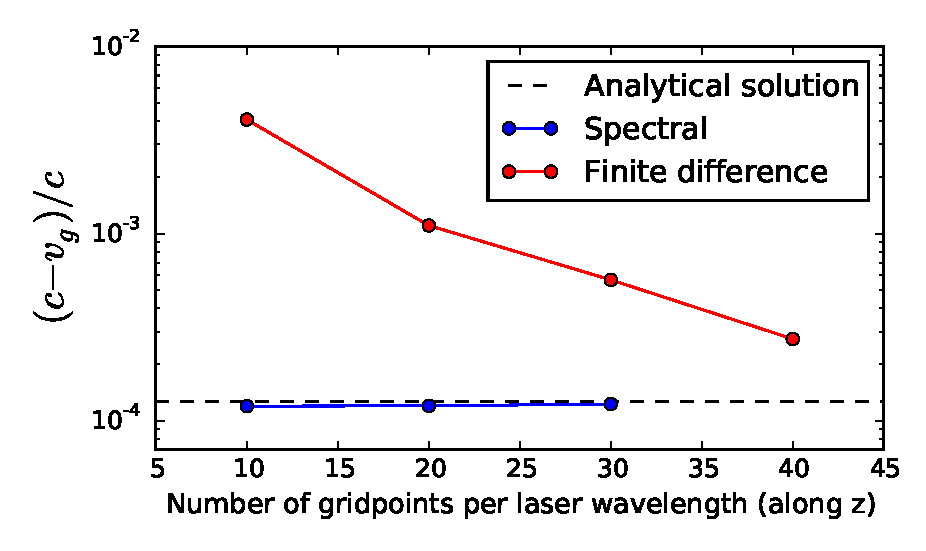
\includegraphics[width=0.6\textwidth]{figures/Vacuum_vg.pdf}
\caption{\label{fig:Vacuum_vg}Relative difference between $c$ and the
group velocity of a laser pulse in vacuum, for different resolutions. The dashed line represents
the analytical prediction given by \cref{eq:vacuum_vg}, while the blue
and red points represent the results of PIC simulation, with the
spectral and finite-difference algorithm.}
\end{figure}


\subsection{Linear propagation in a plasma}
\label{sec:linear_plasma}

In order to confirm that the spectral algorithm also performs well in
the presence of a plasma, we ran the same type of simulations with a
uniform, pre-ionized plasma. The numerical parameters of the
simulations, as well as the physical parameters of the laser, 
were the same as in the previous subsection
(\cref{sec:vacuum_vg}). The plasma was represented by 16
macroparticles per cell, and had a density $n_e = 1.75\times
10^{18}\;\mathrm{cm}^{-3} = 10^{-3}\,n_c$, where $n_c$ is the critical
density for $\lambda=0.8\mathrm{\mu m}$.

Since the intensity of the laser is very low here ($a_0 = 10^{-2}$),
the propagation is linear, and the on-axis group velocity is given by
(e.g. \citep{Esarey1999})
\begin{equation} 
\label{eq:plasma_vg}
\frac{c-v_g}{c} = \frac{n_e}{2n_c} + 2\left( \frac{\lambda}{2\pi w_0} \right)^2
\end{equation}

In \cref{fig:Plasma_vg}, we compare this analytical prediction with the group velocity in the
finite-difference and spectral simulations. Again, the
group velocity is resolution-dependent in the finite-difference
algorithm, and it is substantial different than the analytical
prediction even at high resolution. In the spectral code, the group
velocity velocity exhibits a very weak dependence on resolution
(which is likely due to the errors of current deposition and field
gathering on the finite grid). However, its value remains always very
close to the analytical prediction at all resolutions.

\begin{figure}[!h]
\centering
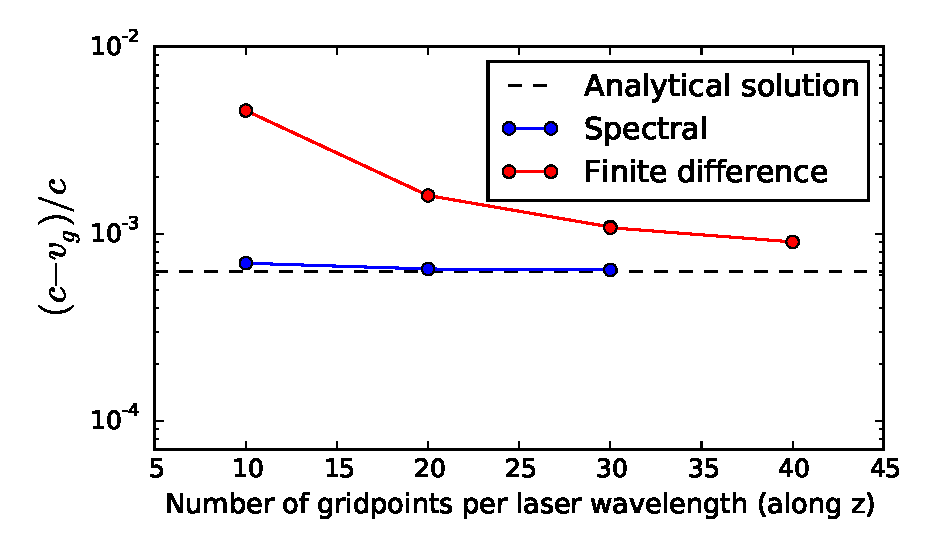
\includegraphics[width=0.6\textwidth]{figures/Plasma_vg.pdf}
\caption{\label{fig:Plasma_vg}Relative difference between $c$ and the
group velocity of a laser pulse in a plasma at $10^{-3}\,n_c$, for different
resolutions. The dashed line represents
the analytical prediction given by \cref{eq:plasma_vg}, while the blue
and red points represent the results of PIC simulation.}
\end{figure}

We emphasize that, although the difference between $c$ and $v_g$ is
small here and may thus seem unimportant, it is this difference which determines
the dephasing length and thus the
maximum beam energy, in a laser-wakefield simulation. It is therefore
paramount to obtain its correct value in the simulation codes. This
problem is well-known in the case of standard finite-difference
codes. For Cartesian finite-difference codes, a common solution is to
use a scheme which is dispersion-free along the $z$ axis 
(e.g. \citep{Karkkainen,Pukhov,Nuter}), but no such scheme has been
developped for quasi-cylindrical codes. Alternatively, numerical dispersion is often 
dealt with in finite-difference codes by either using an even finer grid in
$z$ (which is very computationally expensive) or
a \emph{coarser} grid in $r$. (Recall that, in the simulations shown here, $\Delta r = 5\Delta
z$. A coarser resolution in $r$ allows to
use a larger timestep $\Delta t$, which improves numerical
dispersion.) However, a coarser resolution in $r$ may not always be
adapted to resolve the physics of interest. It is therefore remarkable 
that, with the spectral quasi-cylindrical algorithm, the correct group
velocity is obtained, even for a fine resolution in $r$. 

\subsection{Linear laser-wakefield}

In order to further ascertain that the spectral algorithm described here gives
appropriate results, we ran a simulation of a laser-wakefield, and
compared the amplitude of the wakefield with the corresponding analytical predictions.

In these simulations, the laser was linearly polarized along the
transverse $x$ direction, and had an amplitude $a_0 = 10^{-2}$, a
wavelength $\lambda=0.8 \;\mathrm{\mu m}$, a length $L=10\;\mathrm{\mu
m}$ and a waist $w_0 = 20\;\mathrm{\mu m}$. The simulation was run in
a moving window whose longitudinal and transverse sizes were $80 \;
\mathrm{\mu m}$ and $60 \; \mathrm{\mu m}$. The spatial and temporal
resolutions were $\Delta z = 0.05 \; \mathrm{\mu m}$, $\Delta r = 0.5
\;\mathrm{\mu m}$ and $\Delta t = \Delta z/c$. Since here $a_0 =
10^{-2}$, the analytical wakefield is given by
the linear and quasistatic theory. For a laser of the
form $a(z, r, t)= a_\ell(z, t) e^{-r^2/w_0^2} \cos(k_0z-\omega_0 t)$ --
where $a_\ell(z, t)$ is the longitudinal envelope of the laser -- the
longitudinal and transverse fields $E_z$ and $E_y$ are given by (e.g. \citep{EsareyRMP2009})
\begin{equation} 
E_z(z, r, t) = \frac{mc^2}{e} \frac{k_p^2}{4}\int_{z}^{\infty} 
a_\ell^2(z', t) e^{-r^2/w_0^2} \cos[k_p(z-z')]dz' \label{eq:analytical-Ez}
\end{equation}
\begin{equation}
E_y(z, r, t) = -\frac{mc^2}{e} \frac{k_p y}{w_0^2}\int_{z}^{\infty} 
a_\ell^2(z', t) e^{-r^2/w_0^2} \sin[k_p(z-z')]dz' \label{eq:analytical-Ey}
\end{equation}
\noindent where $k_p$ is the plasma wavevector.

Here, the longitudinal laser envelope $a_\ell$ was extracted directly from the
simulation, and the above analytical integrals where carried out
numerically. The resulting predicted fields $E_z$ and $E_y$ are plotted in dashed lines
in the left and right lower panels of \cref{fig:Linear_wkfld}
respectively. These predicted curves are compared with
the fields $E_z$ and $E_y$ extracted directly from the simulation (red
lines in the lower panels). These fields from the simulation are also
displayed as colormaps in the upper panels of \cref{fig:Linear_wkfld},
and these colormaps include the line along which the quantities in the
lower panels are plotted (dashed line).

\begin{figure}[!h]
\centering
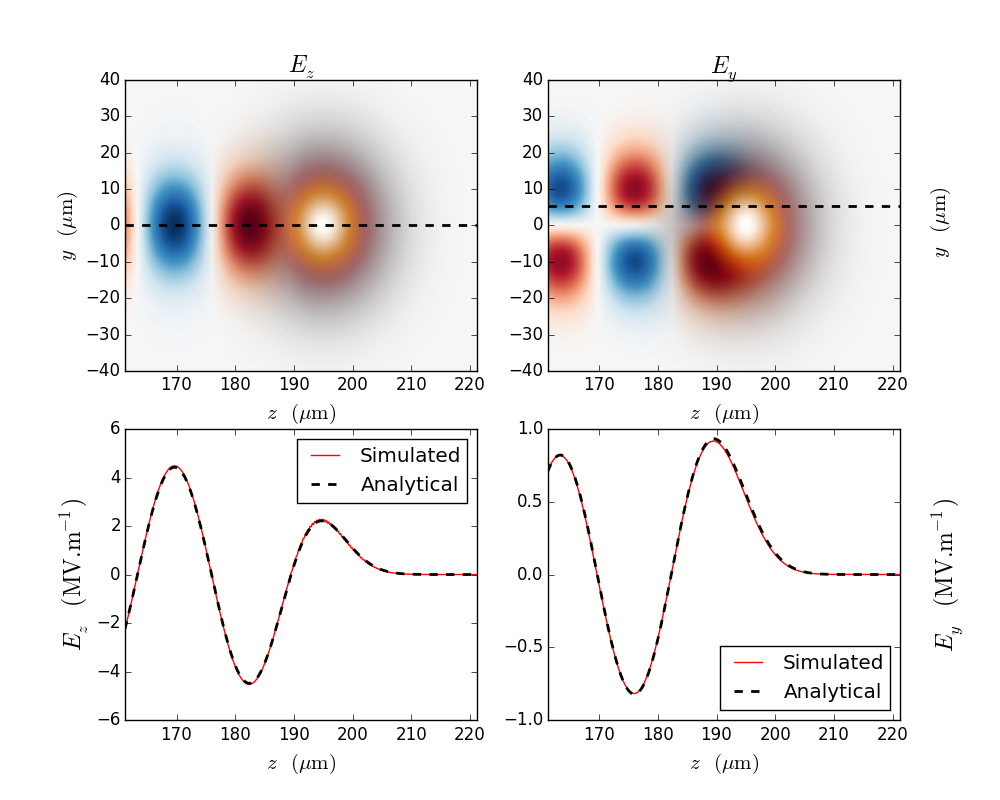
\includegraphics[width=\textwidth]{figures/Linear_wkfld.png}
\caption{\label{fig:Linear_wkfld}Upper panels: Colormaps of the fields $E_z$ and
  $E_y$ as extracted from the simulation (blue and red), along with
  the laser enveloppe (orange hues). (The laser propagates to the
  right and is polarized along $x$.) The dashed lines indicate the
  position where the curves of the lower panels have been extracted. 
Lower panels: profile of the fields at a given radial
position, as given by \cref{eq:analytical-Ez,eq:analytical-Ey} (dashed
line) and extracted from the simulation (red line).}
\end{figure}

As can be seen on the lower panels of \cref{fig:Linear_wkfld}, the
analytical and simulated curves overlap very precisely, which confirms
the validity of our PIC algorithm. This agreement is all
the more remarkable as the $E_z$ field has been extracted from the cells
that are closest to the axis, a region where quasi-cylindrical algorithms
are typically very noisy.


\section{Advantages over finite-difference algorithms}
\label{sec:advantages}

Since finite-difference algorithms and spectral algorithms are
considerably different, each of them have their own advantages and
shortcomings. 

For instance, spectral algorithms -- including the one described here
-- are generally more difficult to parallelize than finite-difference
codes. Similarly, the implementation of specific boundary
conditions, and of a moving window, is usually more challenging in a
spectral algorithm. On the other hand, due to their high precision,
spectral algorithms can avoid a
number of numerical artifacts that are typically present in
finite-difference algorithms. This is quite important as, in a
finite-difference simulation, these artifacts may remain unnoticed
unless additional care is taken in their analysis, and yet they may
affect the physics at stake in an important way.

One example of such an artifact is numerical dispersion, which, as
mentioned in \citep{CowanPRSTAB2013} and in \cref{sec:linear_plasma}, 
can modify the dephasing length of a laser-wakefield accelerator -- a
spurious effect which
may be difficult to discern, especially in the cases where there is no
analytical formula for this length. As shown in
\cref{sec:linear_plasma}, the algorithm described here would not suffer
from this effect, as it is free of numerical dispersion. Similarly, in
this section, we describe two other typical situations in which our spectral
quasi-cylindrical algorithm avoids important artifacts, that would otherwise
arise in a finite-difference code. 

\subsection{Absence of numerical Cherenkov radiation 
for lab-frame simulations}

\comment{Look at spectrum + mitigate claims}

A first artifact which is avoided, in the case of lab-frame
simulations, is numerical Cherenkov radiation. Numerical
Cherenkov radiation is a consequence of numerical dispersion
\citep{GodfreyJCP1974}, and arises because some relativistic particles can
travel faster than the numerically-altered speed of the
electromagnetic waves, in the simulations. This typically causes these
relativistic particles to emit a characteristic spurious
radiation. Recently, it was shown that this spurious radiation
can have a very substantial impact in
lab-frame simulations of laser-wakefield acceleration, 
in particular by increasing the
emittance of the simulated accelerated beam \citep{LehePRSTAB2013}. It
was also shown that, by modifying the PIC algorithm and its
numerical dispersion relation, Cherenkov radiation could be
suppressed. (We note that, in the case of boosted frame simulations,
more complicated secondary numerical Cherenkov effects can develop, 
which are not as easily suppressed \citep{XuJCP2013,YuJCP2014,YuCPC2015,
GodfreyIEEE2014,GodfreyJCP2014}. However, these secondary effects seem not to
have enough time to develop in the case of typical lab-frame simulations.) 

Since the spectral quasi-cylindrical algorithm described here is
dispersion-free, it should not exhibit numerical Cherenkov
radiation in the lab-frame. In order to confirm this prediction, we ran a simulation of
laser-wakefield acceleration with our spectral quasi-cylindrical
algorithm, and compared it with an equivalent simulation that uses 
the finite-difference quasi-cylindrical algorithm of \textsc{Warp}.

In these simulations, a laser pulse with a waist $w_0 = 16\;\mathrm{\mu m}$,
a length $L=10\;\mathrm{\mu m}$, an amplitude $a_0 = 4$ and a
wavelength $\lambda = 0.8\;\mathrm{\mu m}$
is sent into a longitudinally-shaped pre-ionized gas jet. The gas jet
has a 200 $\mathrm{\mu m}$-long rising density gradient at its
entrance, followed by a 200 $\mathrm{\mu m}$ plateau at a density $n_e = 1 \times
 10^{18}\;\mathrm{cm^{-3}}$ and then by a 200 $\mathrm{\mu m}$-long
 downramp, so as to finally reach a density $n_e = 0.5 \times
 10^{18}\;\mathrm{cm^{-3}}$. The downramp causes the injection of an
 electron beam, which is then accelerated in the subsequent density 
plateau at $n_e = 0.5 \times 10^{18}\;\mathrm{cm^{-3}}$. 
Both the spectral and the finite-difference simulations were run in a moving
window whose longitudinal and transverse dimensions were 160 $\mathrm{\mu
  m}$ and 48 $\mathrm{\mu m}$, and both simulations used a resolution
$\Delta z = 0.032 \; \mathrm{\mu m}$ and $\Delta r = 0.19 \; \mathrm{\mu
  m}$. Again, the finite-difference simulation was run with a timestep
$c\Delta t = 1/\sqrt{1/\Delta z^2 + 2/\Delta r^2}$ while the spectral
simulation was run with $c\Delta t = \Delta z$. Importantly, the
charge and currents are smoothed in both
simulations. The spectral algorithms performs smoothing in spectral
space as described in \cref{sec:current-deposition}, while the finite-difference
algorithm applies a single-pass binomial filter on the spatial grid,
in both the $z$ and $r$ directions.

\Cref{fig:Cherenkov} shows a snapshot of the two
simulations, at a similar physical time. The red colormap represents the quantity
$|E_y+cB_x|$, while the superimposed shades of blue represent the electron density. (The
quantity $E_y+cB_x$ is chosen because it corresponds to the $y$ component of
the Lorentz force $\vec{F} = q\vec{E} + q\vec{v}\times\vec{B}$ felt by
a relativistic electron having $\vec{v} = c\vec{e_z}$.) As can be seen
in the top panels, the global aspect of the bubble and of the injected
bunch is similar in both simulations. In particular, the injected
charge was found to be almost the same (766~pC with the
finite-difference algorithm and 750~pC with the spectral
algorithm). However, when having a closer look at the bunch in the
finite-difference algorithm (see the lower left panel in
\cref{fig:Cherenkov}), it appears that the bunch emits a
high-frequency radiation. This radiation is characteristic of the
numerical Cherenkov effect \citep{LehePRSTAB2013}, and is
unphysical. Importantly, the amplitude of this unphysical field
happens to be comparable to the focusing
fields inside the bubble, and it can thus potentially affect the bunch
in a substantial manner. On the other hand, the spectral algorithm does not
exhibit this unphysical radiation (see the lower right panel in
\cref{fig:Cherenkov}), as expected from its dispersion-free property. 
This confirms the fact that, in the lab frame, our spectral
quasi-cylindrical algorithm is free of
the unphysical artifacts associated with numerical Cherenkov radiation.

\begin{figure}[!h]
\centering
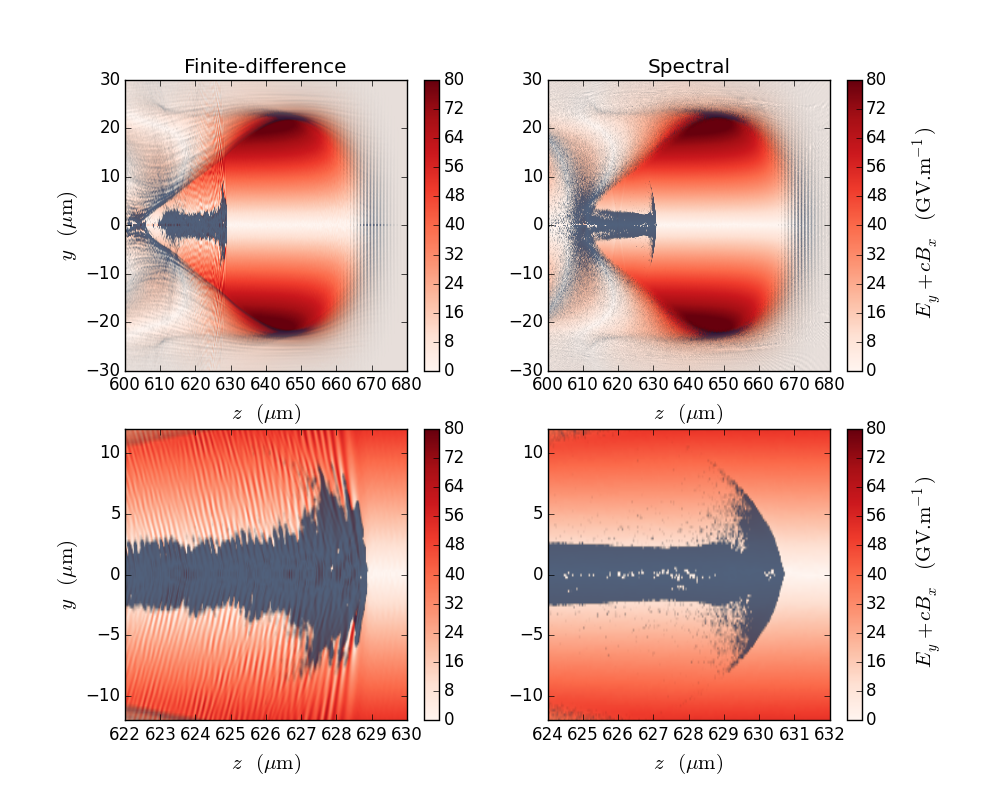
\includegraphics[width=\textwidth]{figures/Cherenkov.png}
\caption{\label{fig:Cherenkov}Snapshot of a finite-difference
  simulation (left) and of a spectral simulation (right), at a similar
  physical time. The superimposed blue shades represent the electron
  density. The lower panels show the region surrounding the
  bunch in more details.}
\end{figure}

For completeness, we remark that a similar suppression of the
numerical Cherenkov radiation was 
obtained in \citep{LehePRSTAB2013,CowanPRSTAB2013}, by using 
modified finite-difference algorithms. However, it is important to
note that these algorithms were applicable to a Cartesian PIC code,
but not to a quasi-cylindrical code. An adaptation to
cylindrical geometry is proposed in \citep{LeheThesis}, and was 
shown to efficiently suppress numerical Cherenkov. However, this
adaptation is not, strictly speaking, dispersion-free. 

\subsection{Accurate force of a laser on a copropagating electron}
\label{sec:accurate-laser}

Another case in which our spectral algorithm performs better than
finite-difference algorithms is whenever a relativistic electron bunch
overlaps with a copropagating laser. This situation occurs for
instance in laser-wakefield acceleration, when the accelerated electron bunch
progressively catches up with the laser pulse and may eventually
overlap with it (e.g. \citep{CipicciaNatPhys2011,NemethPRL2008}). It is also the typical
configuration for simulations of free-electron lasers, where the
overlap of the electron bunch and the copropagating laser radiation, inside an
undulator, leads to a growing instability.

Despite the practical importance of this physical configuration, it
was recently shown that standard finite-difference PIC codes tend 
to largely overestimate the force felt by the electrons inside a
copropagating laser (see the appendix of \citep{LehePRSTAB2014}). This
overestimation was shown to be mainly due to the staggering in time 
of the $\vec{E}$ and $\vec{B}$ fields in a standard finite-difference
code. This staggering indeed results in an improper numerical compensation of 
the two terms of the Lorentz force $\vec{F} = q\vec{E} +
q\vec{v}\times\vec{B}$. However, in our spectral quasi-cylindrical
algorithm, the fields $\vec{E}$ and $\vec{B}$ are not staggered in
time, and thus the force on a copropagating electron bunch should be
correct.

To confirm this prediction, we ran a test simulation in which a single
relativistic macroparticle copropagates with a laser pulse. The initial configuration of
the simulation is represented in \cref{fig:Schematic_laser}. The laser
pulse is polarized along $x$ and is characterized by a waist $w_0 = 25\;\mathrm{\mu m}$,
a length $L=7\;\mathrm{\mu m}$, an amplitude $a_0 = 0.2$ and a
wavelength $\lambda = 0.8\;\mathrm{\mu m}$, while the macroparticle
represents a relativistic electron having an initial Lorentz factor
$\gamma_e = 25$. For comparison, the simulation was run, again, with both our spectral
quasi-cylindrical algorithm and the finite-difference
quasi-cylindrical algorithm of \textsc{Warp}. In order to study
numerical convergence, the simulations were run with a varying
longitudinal resolution $\Delta z$, but with fixed cell aspect ratio
$\Delta r = 10\Delta z$. The timestep was again $c\Delta t=
1/\sqrt{1/\Delta z^2 + 2/\Delta r^2}$ for the finite-difference
simulation and $c\Delta t = \Delta z$ for the spectral
simulation. Finally, the simulations were run in a moving window with a
longitudinal and transverse size of 40 $\mathrm{\mu m}$ and 60 
$\mathrm{\mu m}$ respectively.

\begin{figure}[!h]
\centering
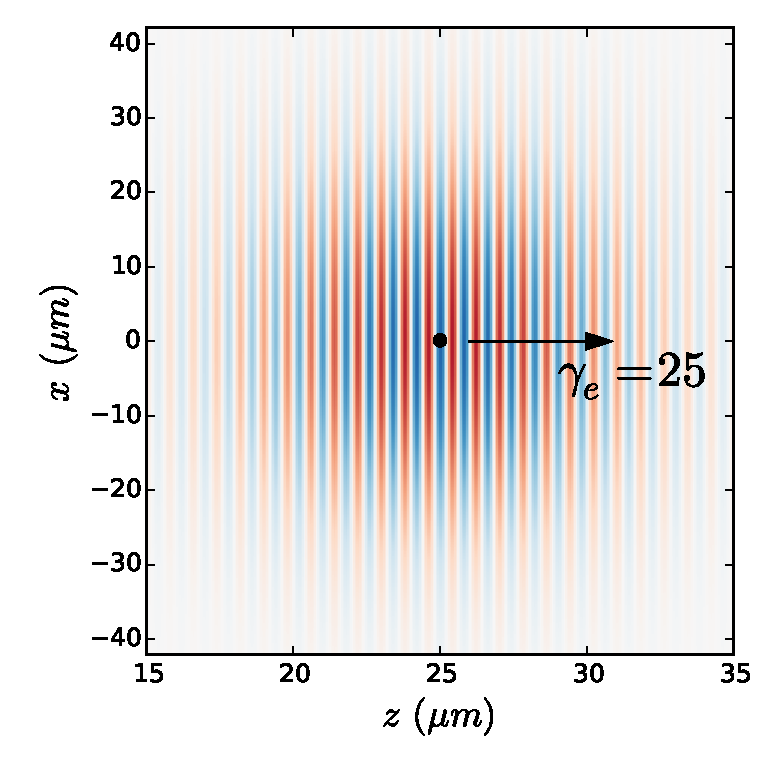
\includegraphics[width=0.5\textwidth]{figures/Schematic_laser.pdf}
\caption{\label{fig:Schematic_laser}Representation of the situation
  which is simulated in \cref{sec:accurate-laser}. The red and blue
  colormap corresponds to the electric field of the laser pulse, while
  the black dot corresponds to the electron considered. 
The laser propagates to the right, and is polarized along $x$.}
\end{figure}

In order to assess the correctness of the force felt by the electron,
we analyzed the evolution of its transverse momentum in
time. Analytically, it can be shown from the Lagrangian 
$\mathcal{L} = - \sqrt{1-\vec{\beta}^2} \,mc^2 - e \vec{v} \cdot
\vec{A}$ that the equation of motion along the $x$ axis (i.e. the axis of laser polarization) is 
\[ \frac{1}{c}\frac{d \,}{dt} \left( \frac{p_x}{m_e c} - a_x \right) =
 - \frac{p_x}{\gamma m_e c}\frac{\partial a_x}{\partial x} \qquad \sim
\frac{a_0^2}{\gamma w_0} \]
\noindent where $a_x$ is the normalized vector potential of the laser
pulse. The right-hand side corresponds to the ponderomotive force, and,
for the parameters and timescale considered here, it is in fact
negligible. The canonical momentum of the
electron is thus approximately conserved.
\[ \frac{p_x}{m_e c} - a_x  = const. \]
\noindent Since, inside the laser pulse, $a_x$ oscillates between the values $-a_0$ and $a_0$,
the quantity $p_x/m_e c$ is predicted to also also oscillate
between $-a_0$ and $a_0$, as the electron progressively
dephases with the laser. 

Keeping in mind that here initially $a_0=0.2$, one can observe on
\cref{fig:Laser} that the oscillation amplitude of $p_x/m_e c$
is much higher than analytically predicted, in the finite-difference
simulation. In addition, these oscillations strongly depend on the
resolution of the simulation, which confirms their spurious nature. These
observations are consistent with those of \citep{LehePRSTAB2014}, and
they are due to the above-mentioned erroneous calculation of the
Lorentz force. On the other hand, in the spectral simulations, the
evolution of $p_x/m_e c$ exhibits virtually no dependence on the
resolution. In addition, the oscillations of $p_x/m_e c$ have a realistic
amplitude. (The fact that these oscillations do not reach exactly the
value 0.2 may be due to the fact that $a_0$ decreases as the laser
propagates, as a consequence of diffraction.) These observations
confirm that the spectral quasi-cylindrical algorithm properly calculates
the Lorentz force on the electron. This is also consistent with our
expectations, which were based on the fact that $\vec{E}$ and $\vec{B}$ are not
staggered in time.

\begin{figure}[!h]
\centering
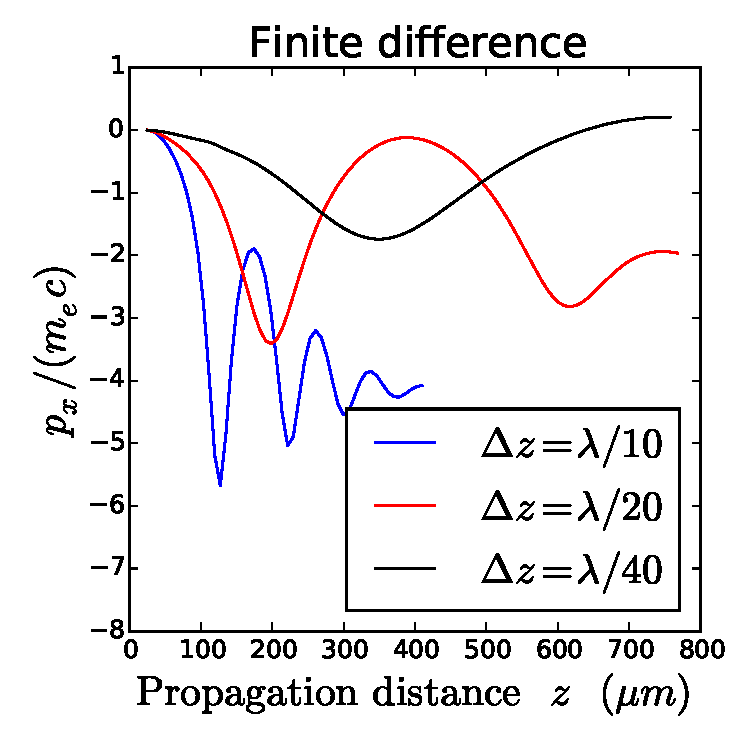
\includegraphics[width=0.45\textwidth]{figures/Laser_finite-difference.pdf}
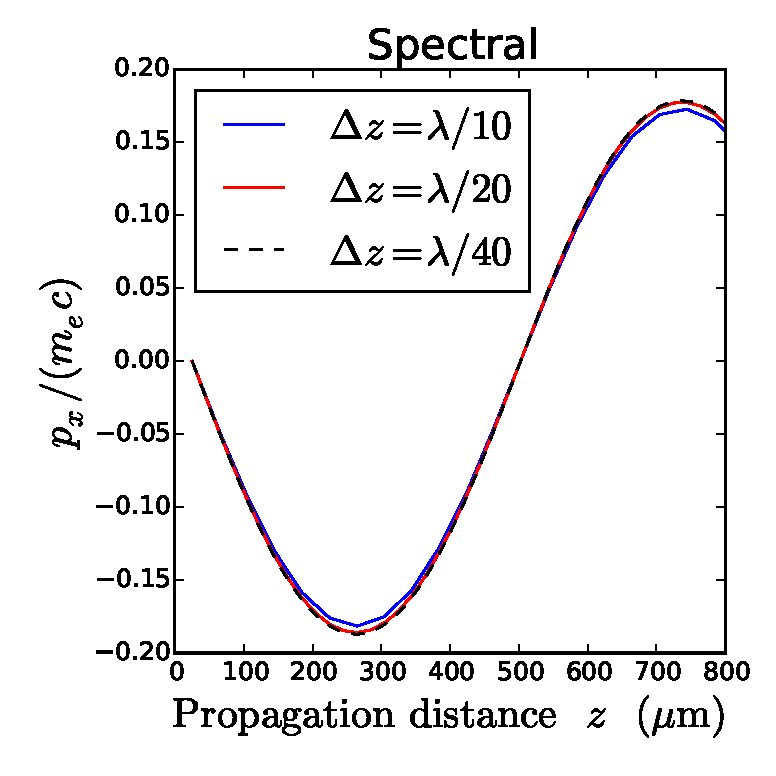
\includegraphics[width=0.45\textwidth]{figures/Laser_spectral.pdf}
\caption{\label{fig:Laser}Evolution of the transverse normalized
  momentum of a macroparticle, as it copropagates with a
  laser pulse having $a_0 = 0.2$ (see \cref{fig:Schematic_laser} for a
  schematic representation of the situation simulated). The left and
  right plots correspond to the finite-difference and spectral
  algorithm respectively (note the different vertical scales on the two
  plots). The colored curves correspond to different resolutions for the simulations.}
\end{figure}


\section*{Conclusion}

In this article, we derived the equations of a spectral
quasi-cylindrical PIC algorithm, and discussed its numerical
implementation. As explained in the text, because this algorithm is
quasi-cylindrical, it require much less computational
time and memory than a full 3D algorithm. In addition, the fact
that it is spectral (and uses the PSATD algorithm) prevents a certain number of
artifacts, that are usually present in a finite-difference algorithm.

This second aspect was tested in details in this article, through
several benchmarks. By comparing simulations with analytical results, 
we showed that our spectral quasi-cylindrical code is free of
numerical dispersion, that it does not exhibit numerical Cherenkov radiation in typical lab-frame
simulations, and that it can accurately calculate the force of a
laser on a copropagating electron. By running the
same benchmarks with a finite-difference quasi-cylindrical algorithm, we showed that
these numerical artifacts could, on the contrary, be present in
finite-difference PIC algorithms. 

However, it must not be forgotten that
finite-difference algorithms have advantages of their own, including
easier parallelization and application of boundary conditions. In the
case of our spectral quasi-cylindrical algorithm, parallelization to
several nodes could nonetheless be achieved by following for instance the
method of \citep{VayJCP2013}. This will be the subject of future work. 

\paragraph{Acknowledgements}

We thank Axel Huebl for interesting discussions on the GPU implementation.

This work was supported by the Director, Office of Science, Office of High Energy Physics, U.S. Dept. of Energy under Contract No. DE-AC02-05CH11231, including from the Laboratory Directed Research and Development (LDRD) funding from Berkeley Lab.

This document was prepared as an account of work sponsored in part by the United States Government. While this document is believed to contain correct information, neither the United States Government nor any agency thereof, nor The Regents of the University of California, nor any of their employees, nor the authors makes any warranty, express or implied, or assumes any legal responsibility for the accuracy, completeness, or usefulness of any information, apparatus, product, or process disclosed, or represents that its use would not infringe privately owned rights. Reference herein to any specific commercial product, process, or service by its trade name, trademark, manufacturer, or otherwise, does not necessarily constitute or imply its endorsement, recommendation, or favoring by the United States Government or any agency thereof, or The Regents of the University of California. The views and opinions of authors expressed herein do not necessarily state or reflect those of the United States Government or any agency thereof or The Regents of the University of California.

\newpage
\appendix


\section{Derivation of the Fourier-Bessel representation}
\label{sec:CircTrans}

In order to derive the representation \cref{eq:CircBwTrans} we have to
distinguish the fields that are well-defined everywhere in space (like
$E_x$, $E_y$, $E_z$, $B_x$, $B_y$, $B_z$) and thus have a regular
Fourier representation, from those that are ill-defined at $r=0$ (like $E_r$, $E_\theta$, $B_r$, $B_\theta$).

\subsection{Fields that are well-defined everywhere}

Let $F_u$ be a field that is well-defined everywhere in space
(typically $F$ is $E$, $B$ or $J$ and $u$ is $x$, $y$ or $z$). Its Fourier representation
is thus given by \cref{eq:CartBwTrans,eq:CartFwTrans}:
\begin{align*}
F_u(\vec{r}) = \frac{1}{(2\pi)^{3/2}}\Integ{k_x} \,\Integ{k_y}\,
\Integ{k_z} \; \hat{F_u}(\vec{k}) e^{i(k_x x + k_y y + k_z z)} \\
\hat{F_u}(\vec{k})  = \frac{1}{(2\pi)^{3/2}}\Integ{x} \,\Integ{y}\,
\Integ{z} \; F_u(\vec{r}) e^{-i(k_x x + k_y y + k_z z)} 
\end{align*}
Using the change of variable $k_x=k_\perp\cos(\phi)$, $k_y = k_\perp\sin(\phi)$,
$x=r\cos(\theta)$, $y=r\sin(\theta)$, this becomes
 \begin{align*}
F_u(\vec{r}) = \frac{1}{(2\pi)^{3/2}}\Integ{k_z} \,\RInteg{k_\perp}\,
\TInteg{\phi} \; \hat{F_u}(\vec{k})
e^{i(k_\perp r \cos(\theta-\phi) + k_z z)} \\
\hat{F_u}(\vec{k})   = \frac{1}{(2\pi)^{3/2}}\Integ{z} \,\RInteg{r}\,
\Integ{\theta} \; F_u(\vec{r}) e^{-i(k_\perp r \cos(\theta-\phi) + k_z z)} 
\end{align*}
We now use the relation $e^{ik_\perp r\cos(\theta-\phi)} =
\sum_{m=-\infty}^{\infty} i^m J_m(k_\perp r) e^{im(\phi-\theta)}$ in these equations, to obtain
\begin{align*}
F_u (\vec{r})  = \sum_{m=-\infty}^{\infty} \frac{1}{(2\pi)^{3/2}}\Integ{k_z} \,\RInteg{k_\perp }
\TInteg{\phi} \; i^m \hat{F_u}(\vec{k}) \;
J_m(k_\perp r) e^{-im(\theta-\phi) + ik_z z} \\
\hat{F_u}(\vec{k})   =  \sum_{m=-\infty}^{\infty} \frac{1}{(2\pi)^{3/2}}\Integ{z} \,\RInteg{r}
\TInteg{\theta} \;\; (-i)^m F_u(\vec{r}) \; J_m(k_\perp r) e^{-im(\phi-\theta) -ik_z z} 
\end{align*}
We now define $\tilde{F}_{u,m}(k_z,k_\perp ) = \frac{1}{(2\pi)^{3/2}}\int_0^{2\pi}
\mathrm{d}\phi \; i^m \hat{F_u}(\vec{k})
e^{im\phi}$. This results in the following equations :
\begin{align*}
F_u(\vec{r}) = \sum_{m=-\infty}^{\infty} \Integ{k_z}
\RInteg{k_\perp }\; \tilde{F}_{u,m}(k_z,k_\perp ) \; J_m(k_\perp r) e^{-im\theta + ik_z z} 
\\
\tilde{F}_{u,m}(k_z,k_\perp ) = \frac{1}{(2\pi)^2} \Integ{z} \RInteg{r}
\TInteg{\theta} \;F_u(\vec{r})\; J_m(k_\perp r) e^{-im\theta
 - i k_z z}
\end{align*}
These equations correspond to \cref{eq:CircBwTransz,eq:CircFwTransz}.

\subsection{Fields that are ill-defined at $r=0$}

Let us now consider fields of the type $E_r$, $B_r$ or $J_r$, which we
denote generally by $F_r$. We have :
\[ F_r = \cos(\theta) F_x + \sin(\theta) F_y 
= \frac{F_x - iF_y}{2}e^{i\theta} + \frac{F_x +
  iF_y}{2}e^{-i\theta} \] 
Using \cref{eq:CircBwTransu,eq:CircFwTransu}, this leads to
\begin{align} 
F_r =  \sum_{m=-\infty}^{\infty} \Integ{k_z}\,\RInteg{k_\perp }\;
\left(  J_m(k_\perp r) \frac{\tilde{F}_{x,m} -
    i\tilde{F}_{y,m}}{2}e^{-i(m-1)\theta +ik_z z} + J_m(k_\perp r)
  \frac{\tilde{F}_{x,m} +   i\tilde{F}_{y,m}}{2}e^{-i(m+1)\theta +
    ik_z z} \right) \\
= \sum_{m=-\infty}^{\infty} \Integ{k_z}\,\RInteg{k_\perp }\;
\left(  J_{m+1}(k_\perp r) \frac{\tilde{F}_{x,m+1} -
    i\tilde{F}_{y,m+1}}{2}e^{-im\theta +ik_z z} + J_{m-1}(k_\perp r)
  \frac{\tilde{F}_{x,m-1} +   i\tilde{F}_{y,m-1}}{2}e^{-im\theta +
    ik_z z} \right) 
\end{align}
where we relabeled the dummy variable $m$ in the above sums. Let us
thus define $\tilde{F}_{-,m} = \frac{\tilde{F}_{x,m-1} +
    i\tilde{F}_{y,m-1}}{2}$ and $\tilde{F}_{+,m} = \frac{\tilde{F}_{x,m+1} -
    i\tilde{F}_{y,m+1}}{2}$. This results in:
\begin{equation} 
F_r(\vec{r}) = \sum_{m=-\infty}^{\infty} \Integ{k_z}\,\RInteg{k_\perp }\;
\left( \tilde{F}_{+,m}\; J_{m+1}(k_\perp r) +\tilde{F}_{-,m}\; J_{m-1}(k_\perp r)
\right)  e^{-im\theta +ik_z z}
\end{equation}

With the same definitions and the same method, it is also easy to show that:
\begin{equation} 
F_\theta(\vec{r}) = \sum_{m=-\infty}^{\infty} \Integ{k_z}\,\RInteg{k_\perp }\;
i\left( \tilde{F}_{+,m}\; J_{m+1}(k_\perp r) - \tilde{F}_{-,m}\; J_{m-1}(k_\perp r)
\right)  e^{-im\theta +ik_z z}
\end{equation}

\section{Maxwell equations for the spectral coefficients}
\label{sec:SpectMaxwell}

In this section, let us derive the Maxwell equations for the spectral
coefficients \cref{eq:CircMaxwellp,eq:CircMaxwellm,eq:CircMaxwellz}
from the Maxwell equations written in cylindrical coordinates \cref{eq:CircMaxwellr,eq:CircMaxwellt,eq:CircMaxwellzz}.

When replacing the Fourier-Bessel decomposition
(\cref{eq:CircBwTransu,eq:CircBwTransr,eq:CircBwTranst}) in the
Maxwell equations \cref{eq:CircMaxwellr,eq:CircMaxwellt,eq:CircMaxwellzz}, we
first notice that the modes proportional to $e^{-im\theta +ik_z z}$ for different
values of $m$ and $k_z$ are not coupled. These different modes can
thus be treated separately. The same cannot be said of the modes
corresponding to different values of $k_\perp $, since they may be coupled
through the Bessel functions $J_m(k_\perp r)$ and their derivatives. 
In the following, we write only the equations corresponding to $\partial_t \vec{B} =
-\vec{\nabla}\times \vec{E}$, since the equation $c^{-2}\partial_t \vec{E} =
\vec{\nabla}\times\vec{B} - \mu_0 \vec{j}$ can be treated very
similarly. These equations become
\begin{align*}
\RInteg{k_\perp } \left[ \; \partial_t \tilde{B}_{+,m}  J_{m+1}(k_\perp r)
  + \partial_t \tilde{B}_{-,m}  J_{m-1}(k_\perp r) \; \right] =&& \\ 
\qquad \RInteg{k_\perp } \left[ \; \tilde{E}_{z,m} \frac{im}{r}
  J_m(k_\perp r) \right.-&\left.
  k_z\tilde{E}_{+,m}J_{m+1}(k_\perp r) + k_z\tilde{E}_{-,m}J_{m-1}(k_\perp r) \;
\right] & \\
\RInteg{k_\perp } \left[ \; \partial_t \tilde{B}_{+,m}  J_{m+1}(k_\perp r)
  - \partial_t \tilde{B}_{-,m}  J_{m-1}(k_\perp r) \; \right] =&& \\
 \RInteg{k_\perp } \left[ \; -k_z\tilde{E}_{+,m}J_{m+1}(k_\perp r)
 \right.-&\left.  k_z\tilde{E}_{-,m}J_{m-1}(k_\perp r) - ik_\perp \tilde{E}_{z,m} J_m'(k_\perp r) \;\right] \\
\RInteg{k_\perp }\; \partial_t \tilde{B}_{z,m}  J_{m}(k_\perp r) =
\RInteg{k_\perp } \left[ \; -ik_\perp
  \tilde{E}_{+,m}\right.&\left(\frac{J_{m+1}(k_\perp r)}{k_\perp r} +
    J_{m+1}'(k_\perp r) \right) + &\\
\left. ik_\perp \tilde{E}_{-,m}\left(\frac{J_{m-1}(k_\perp r)}{k_\perp r} +
    J_{m-1}'(k_\perp r) \right) \right.-&\left. \frac{im}{r} \left( E_{+,m} J_{m+1}(k_\perp r) +
    E_{-,m} J_{m-1}(k_\perp r) \right) \;\right] 
\end{align*}
By taking the sum and difference of the first two equations, and by
rearranging the third equation, we obtain:
\begin{align*}
\RInteg{k_\perp } \; 2 \,\partial_t \tilde{B}_{+,m}  J_{m+1}(k_\perp r) =
\RInteg{k_\perp } \left[ \; ik_\perp \tilde{E}_{z,m} \left( \frac{m}{k_\perp r} J_m(k_\perp r) -
    J_m'(k_\perp r) \right) -2 k_z\tilde{E}_{+,m}J_{m+1}(k_\perp r) \;
\right] \\
\RInteg{k_\perp } \; 2\, \partial_t \tilde{B}_{-,m}  J_{m-1}(k_\perp r) \; =
\RInteg{k_\perp } \left[ \;
   ik_\perp \tilde{E}_{z,m} \left( \frac{m}{k_\perp r} J_m(k_\perp r) +
    J_m'(k_\perp r) \right)  + 2k_z\tilde{E}_{-,m}J_{m-1}(k_\perp r) \;
\right] \\
\RInteg{k_\perp }\; \partial_t \tilde{B}_{z,m}  J_{m}(k_\perp r) =
\RInteg{k_\perp } \left[ \; -ik_\perp \tilde{E}_{+,m}\left(\frac{m+1}{k_\perp r}J_{m+1}(k_\perp r) +
    J_{m+1}'(k_\perp r) \right) \right.\\
\qquad \left. - ik_\perp \tilde{E}_{-,m}\left(\frac{m-1}{k_\perp r}J_{m-1}(k_\perp r) -
    J_{m-1}'(k_\perp r) \right) \right] 
\end{align*}
We can now use the relations $\frac{m}{k_\perp r} J_m(k_\perp r) +
    J_m'(k_\perp r) = J_{m-1}(k_\perp r)$ and $\frac{m}{k_\perp r} J_m(k_\perp r) -
    J_m'(k_\perp r) = J_{m+1}(k_\perp r)$ (see relation 9.1.27 in
    \cite{Abramowitz}), and obtain :
\begin{align*}
\RInteg{k_\perp } \; 2 \,\partial_t \tilde{B}_{+,m}  J_{m+1}(k_\perp r) =
\RInteg{k_\perp } \left[ \; ik_\perp \tilde{E}_{z,m}\,
    J_{m+1}(k_\perp r) -2 k_z\tilde{E}_{+,m}J_{m+1}(k_\perp r) \;
\right] \\
\RInteg{k_\perp } \; 2\, \partial_t \tilde{B}_{-,m}  J_{m-1}(k_\perp r) \; =
\RInteg{k_\perp } \left[ \;
   ik_\perp \tilde{E}_{z,m} \,
    J_{m-1}(k_\perp r) + 2k_z\tilde{E}_{-,m}J_{m-1}(k_\perp r) \;
\right] \\
\RInteg{k_\perp }\; \partial_t \tilde{B}_{z,m}  J_{m}(k_\perp r) =
\RInteg{k_\perp } \left[ \; -ik_\perp \tilde{E}_{+,m} J_{m}(k_\perp r) - ik_\perp \tilde{E}_{-,m}\,J_{m}(k_\perp r) \right] 
\end{align*}
Each equation of the above system contains Bessel functions of only one
given order (either $m+1$, $m-1$ or $m$). This allows to separate the
different $k_\perp $ components, since it the the functions $J_n(k_\perp r)$, for a
fixed $n$ and different values of $k_\perp $, form a basis of the set of real functions:
\begin{align*}
2 \,\partial_t \tilde{B}_{+,m} =
ik_\perp \tilde{E}_{z,m} -2 k_z\tilde{E}_{+,m} \\
2\, \partial_t \tilde{B}_{-,m} = ik_\perp \tilde{E}_{z,m} \,
    + 2k_z\tilde{E}_{-,m} \\
 \partial_t \tilde{B}_{z,m} = -ik_\perp \tilde{E}_{+,m}  - ik_\perp \tilde{E}_{-,m}
\end{align*}

\section{PSATD scheme, in the Fourier-Bessel
  representation}
\label{sec:PSTADderiv}

We use a scheme very similar to that of \cite{Haber}. In this scheme the currents are considered constant over one timestep, and the charge density is considered linear in time.

\subsection{Expressions for $\tilde{B}_m$}

By combining \cref{eq:CircMaxwellp,eq:CircMaxwellm,eq:CircMaxwellz}
and \cref{eq:SpectCons}, one can find the propagation equations for $B$.
\begin{align*}
\partial_t^2 \tilde{B}_{+,m} + c^2(k_\perp ^2+k_z^2) \tilde{B}_{+,m} = 
\mu_0 c^2 \left( - \frac{ik_\perp }{2} \tilde{j}_{z,m} + k_z \tilde{j}_{+,m}
\right) \\
\partial_t^2 \tilde{B}_{-,m} + c^2(k_\perp ^2+k_z^2) \tilde{B}_{-,m} = 
\mu_0 c^2 \left( - \frac{ik_\perp }{2} \tilde{j}_{z,m} - k_z \tilde{j}_{+,m}
\right) \\
\partial_t^2 \tilde{B}_{z,m} + c^2(k_\perp ^2+k_z^2) \tilde{B}_{z,m} =
\mu_0c^2  (ik_\perp  \tilde{j}_{+,m} + ik_\perp \tilde{j}_{-,m} ) 
\end{align*}
Let us integrate these equations for $t\in [n\Delta t, (n+1)\Delta
t]$. In this interval, $\tilde{j}_m(t)$ is constant
and equal to $\tj_m{n+1/2}$, and thus the right-hand side of the above
equations is constant. Using Green functions, the
general solution of a differential equation of the form 
$\partial_t^2 f + \omega^2 f = g_0$, where $g_0$ is a constant, is 
\[ f(t) = f(t_0) \cos[\,\omega (t-t_0)\,] + \partial_t f (t_0) \frac{
  \sin[\,\omega (t-t_0)\,]  }{\omega} + \frac{g_0}{\omega^2} (1-
\cos[\,\omega (t-t_0)\,] ) \]  
We thus use the above expression, with $\omega^2 =c^2(k_\perp^2 +
k_z^2)$, to integrate the fields from $t_0 = n\Delta t$ to $t=(n+1)\Delta t$. In
particular, we use again the Maxwell equations
\cref{eq:CircMaxwellp,eq:CircMaxwellm,eq:CircMaxwellz} to obtain the
expression of $\partial_t \tilde{B}_{m} (t_0)$. This yields:
\begin{align*}
\tB{+}{n+1} = \; & C \tB{+}{n} - 
\frac{S}{\omega}\left(-\frac{ik_\perp }{2} \tE{z}{n} + k_z\tE{+}{n}
\right) + \mu_0 c^2\frac{1-C}{\omega^2} \left( -\frac{ik_\perp }{2}
  \tj{z}{n+1/2} + k_z \tj{+}{n+1/2} \right)& \\
\tB{-}{n+1} =\; & C \tB{-}{n} - 
\frac{S}{\omega}\left(- \frac{ik_\perp }{2} \tE{z}{n} - k_z\tE{-}{n}
\right) + \mu_0 c^2\frac{1-C}{\omega^2} \left( - \frac{ik_\perp }{2}
  \tj{z}{n+1/2} - k_z \tj{-}{n+1/2} \right) &\\
\tB{z}{n+1} =\; & C \tB{z}{n} - 
\frac{S}{\omega}\left(ik_\perp \tE{+}{n} + ik_\perp \tE{-}{n}
\right) + \mu_0 c^2\frac{1-C}{\omega^2} \left( ik_\perp
  \tj{+}{n+1/2} + ik_\perp \tj{-}{n+1/2} \right)&
\end{align*}
where $C = \cos(\omega \Delta t)$ and $S = \sin(\omega \Delta t) $.

\subsection{Expressions for $\tilde{E}_m$}

Similarly, when combining \cref{eq:CircMaxwellp,eq:CircMaxwellm,eq:CircMaxwellz}
and \cref{eq:SpectCons}, the propagation equations for $E$ are:
\begin{align*}
\partial_t^2 \tilde{E}_{+,m} + c^2(k_\perp^2 + k_z^2) \tilde{E}_{+,m}
= \frac{c^2}{\epsilon_0} \frac{k_\perp}{2} \tilde{\rho}_m -
\mu_0c^2 \partial_t\tilde{j}_{+,m} \\
\partial_t^2 \tilde{E}_{-,m} + c^2(k_\perp^2 + k_z^2) \tilde{E}_{-,m}
= - \frac{c^2}{\epsilon_0} \frac{k_\perp}{2} \tilde{\rho}_m -
\mu_0c^2 \partial_t\tilde{j}_{-,m} \\
\partial_t^2 \tilde{E}_{z,m} + c^2(k_\perp^2 + k_z^2) \tilde{E}_{z,m}
= - \frac{c^2}{\epsilon_0} i k_z \tilde{\rho}_m -
\mu_0c^2 \partial_t\tilde{j}_{z,m} 
\end{align*}
Let us again integrate these equations for $t\in [n\Delta t, (n+1)\Delta
t]$. In this interval, $\tilde{j}_m(t)$ is constant (thus its time
derivatives drop), and $\tilde{\rho}_m$ is linear in time. As a
consequence the right hand side is proportional to $\trho{n} +
(\trho{n+1}-\trho{n})(t-t_0)/\Delta t$. Using Green functions, the solution of 
$ \partial_t^2 f + \omega^2 f = \trho{n} + (\trho{n+1}-\trho{n})(t-t_0)/\Delta t $ is
\[ f(t) = f(t_0) \cos[\,\omega(t-t_0)\,] + \partial_tf (t_0)
\frac{\sin[\,\omega(t-t_0)\,]}{\omega} + \trho{n}\frac{1-
  \cos[\,\omega(t-t_0)\,]}{\omega^2} + \frac{\trho{n+1}-\trho{n}}{\omega^2}\left(
  \frac{t-t_0}{\Delta t} - \frac{\sin[\,\omega(t-t_0)\,]}{\omega
    \Delta t}
\right) \]
which, for $t=t_0 +\Delta t$, reduces to
\[ f(t_0 +\Delta t) = f(t_0) C + \partial_tf (t_0)
\frac{S}{\omega} + \trho{n}\frac{S-\omega\Delta t
  C}{\omega^3\Delta t} + \frac{\trho{n+1}}{\omega^2}\left(
  1 - \frac{S}{\omega\Delta t}\right) \]
Using the above expression, we obtain
\begin{align*}
\tE{+}{n+1} = \; & C \tE{+}{n} + 
\frac{S}{\omega}\left(-\frac{ik_\perp }{2} \tB{z}{n} + k_z\tB{+}{n}
- \mu_0 \tj{+}{n+1/2} \right) + \frac{c^2}{\epsilon_0}
\frac{k_\perp}{2}\left[ \trho{n}\frac{S-\omega\Delta t
  C}{\omega^3\Delta t} + \frac{\trho{n+1}}{\omega^2}\left(
  1 - \frac{S}{\omega\Delta t}\right) \right]  & \\
\tE{-}{n+1} =\; & C \tE{-}{n} +
\frac{S}{\omega}\left(- \frac{ik_\perp }{2} \tB{z}{n} - k_z\tB{-}{n}
- \mu_0 \tj{-}{n+1/2} \right) - \frac{c^2}{\epsilon_0}
\frac{k_\perp}{2}\left[ \trho{n}\frac{S-\omega\Delta t
  C}{\omega^3\Delta t} + \frac{\trho{n+1}}{\omega^2}\left(
  1 - \frac{S}{\omega\Delta t}\right) \right]  &\\
\tE{z}{n+1} =\; & C \tE{z}{n} + 
\frac{S}{\omega}\left(ik_\perp \tB{+}{n} + ik_\perp \tB{-}{n}
- \mu_0 \tj{z}{n+1/2} \right) - \frac{c^2}{\epsilon_0}
ik_z\left[ \trho{n}\frac{S-\omega\Delta t
  C}{\omega^3\Delta t} + \frac{\trho{n+1}}{\omega^2}\left(
  1 - \frac{S}{\omega\Delta t}\right) \right]  &
\end{align*}

\section{Discrete Hankel Transform}
\label{sec:HTMatrix}

Say we extend the formulas \cite{Guizar} to the case of a regular
grid in space, and to the case where the order of the transform and
that of the $k$ grid are not the same.

Reminder:
\[ \mathrm{DHT_n}[f] \,(k^m_{\perp,j}) = \sum_{p=0}^{N_r-1} M_{j,p}(n,m)
\,f(r_p) \qquad \mathrm{IDHT_n}[g] \, (r_j) = \sum_{p=0}^{N_r-1}
M^{-1}_{j,p}(n,m) \,g(k^m_{\perp,p}) \]
These matrices can be determined by a set of $N_r^2$ conditions. These
conditions can be found by imposing the value of the DHT for a set of  $N_r$ functions.

In our case, we impose that the DHT be equal to the exact HT for the eigenmodes of a cavity with
perfectly conducting boundary at $r_{max}$ ($E_z(r_{m},z) =
0$), since these physical eigenmodes should also be eigenmodes of our
PIC cycle. These eigenmodes have the following form:
\begin{align*}
E_z \;& \; \propto  J_m(k^m_{\perp,\ell} \,r)\,e^{ik_z z -im\theta} \Theta(r_{max}-r) \\
E_r -i E_\theta \;& \; \propto  J_{m+1}(k^m_{\perp,\ell} \,r) \,e^{ik_z z -im\theta} \Theta(r_{max}-r)\\
E_r +i E_\theta \;& \; \propto  J_{m-1}(k^m_{\perp,\ell} \,r) \,e^{ik_z z -im\theta} \Theta(r_{max}-r) 
\end{align*}
where $\Theta$ is the Heaviside function and where $k^m_{\perp,\ell} =
\alpha^m_\ell / r_{max}$, with $\alpha^m_j$ the $j$th strictly positive zero of
the Bessel function of order $m$. They form an othogonal basis of
functions for this chosen boundary condition. The exact Hankel transform of these modes, evaluated on the discrete set $\{
k^m_{\perp,j} \}$ reads (see relation 11.4.5 in \cite{Abramowitz}).
\begin{align*} 
\mathrm{HT}_{m}[ \; J_m(k^m_{\perp,\ell} \,r) \;] \,(k^m_{\perp,j} )
&\quad \equiv 2\pi \rInteg \; J_m (k^m_{\perp,\ell} r) J_m (k^m_{\perp,j} r)
&\quad = \pi\, r_{max}^2\,[ J_{m+1}(\alpha_j^m)]^2 \; \delta_{j,\ell} \\
\mathrm{HT}_{m+1}[ \; J_{m+1}(k^m_{\perp,\ell} \,r) \;] \,(k^m_{\perp,j} )
&\quad \equiv 2\pi \rInteg \; J_{m+1} (k^m_{\perp,\ell} r)
  J_{m+1}(k^m_{\perp,j} r) 
&\quad = \pi\, r_{max}^2\,[ J_{m+1}(\alpha_j^m)]^2 \; \delta_{j,\ell} \\
\mathrm{HT}_{m-1}[ \; J_{m-1}(k^m_{\perp,\ell} \,r) \;] \,(k^m_{\perp,j} )
& \quad \equiv 2\pi \rInteg \; J_{m-1} (k^m_{\perp,\ell} r) J_{m-1} (k^m_{\perp,j}
  r) 
&\quad = \pi\, r_{max}^2\,[ J_{m+1}(\alpha_j^m)]^2 \; \delta_{j,\ell}
\end{align*}
\textbf{Explain more why we want these functions to be
  preserved. Explain why we take (m+1) and (m-1)}

Here we impose that the DHT of these functions has the same value for $(j,\ell) \in \{ 0,
..., N_r - 1\}$
\begin{align*}
\mathrm{DHT}_{m}[ \; J_m(k^m_{\perp,\ell} \,r) \;] \,(k^m_{\perp,j}) 
&\quad \equiv \sum_{p=0}^{N_r-1} M_{j,p}(m,m)
  J_m(k^m_{\perp,\ell}\,r_p) 
&\quad = \pi\, r_{max}^2\,[ J_{m+1}(\alpha_j^m)]^2 \; \delta_{j,\ell} \\
\mathrm{DHT}_{m+1}[ \; J_{m+1}(k^m_{\perp,\ell} \,r) \;]\,(k^m_{\perp,j})
&\quad \equiv \sum_{p=0}^{N_r-1} M_{j,p}(m+1,m)
  J_{m+1}(k^m_{\perp,\ell}\,r_p) 
&\quad = \pi\, r_{max}^2\,[ J_{m+1}(\alpha_j^m)]^2 \; \delta_{j,\ell} \\
\mathrm{DHT}_{m-1}[ \; J_{m-1}(k^m_{\perp,\ell} \,r) \;] \,(k^m_{\perp,j})
& \quad \equiv \sum_{p=0}^{N_r-1} M_{j,p}(m-1,m)
 J_{m-1}(k^m_{\perp,\ell}\,r_p) 
&\quad = \pi\, r_{max}^2\,[ J_{m+1}(\alpha_j^m)]^2 \; \delta_{j,\ell}
\end{align*}
The above relations impose $N_r^2$ conditions on the matrices
$M(m,m)$, $M(m+1,m)$, $M(m-1,m)$ and thus allows one to completely
determine them. In fact, a closer look at the above relations shows
that the inverse matrices $M^{-1}(m,m)$, $M^{-1}(m+1,m)$,
$M^{-1}(m-1,m)$ can be directly extracted from the above relations,
since these inverse matrices are defined by the relation $\sum_p M_{j,p}(n,m)
M^{-1}_{p,\ell}(n,m) = \delta_{j,\ell}$. Indeed, from the above
relations, one can directly infer:
\[ M^{-1}_{p,\ell}(m,m) = \frac{ J_m(k^m_{\perp,\ell}\,r_p) } { \pi\,
  r_{max}^2\,[ J_{m+1}(\alpha_j^m)]^2  } \]
\[ M^{-1}_{p,\ell}(m \pm 1,m) = \frac{ J_{m\pm 1}(k^m_{\perp,\ell}\,r_p) } { \pi\,
  r_{max}^2\,[ J_{m+1}(\alpha_j^m)]^2  } \]
The matrices $M(m,m)$, $M(m+1,m)$, $M(m-1,m)$ can then be extracted,
by numerically inverting the matrices  $M^{-1}(m,m)$, $M^{-1}(m+1,m)$,
$M^{-1}(m-1,m)$ given by the above expressions.

\bibliography{Bibliography}
\bibliographystyle{elsarticle-harv}

\end{document}
